\chapter{Di-$b$-Jet Search: Limit Setting Phase}
\label{sec:lim}

In Chapter~\ref{sec:bkg} it was shown that there is no evidence of new physics in the dijet mass spectra of the observed di-$b$-jet events
\footnote{\ Defined as events that pass the di-$b$-jet event selection.}. %%%%% This is reference by hand later!!!! Change below if changing this.
However, it is also useful to quantify what this result means in the context
of the signal models that are being searched for.
Specifically, one can estimate the degree of belief that a signal model is true given the di-$b$-jet events that have been observed.
If the degree of belief in a specific model is less than a certain threshold the model is excluded.
This process is known as the limit setting phase.

In this Chapter,
Section~\ref{sec:lim-strat} will describe the limit setting methodology and
Section~\ref{sec:lim-syst} will discuss the systematic uncertainties considered.
Then Sections~\ref{sec:lim-summer}~and~\ref{sec:lim-full} present the details and
the results of the limit setting phase for the \summer{} and \lm{} data-sets respectively.

\section{Limit Setting Methodology}
\label{sec:lim-strat}

In this analysis a Bayesian limit setting approach is used~\cite{det-thesis_kate,lim-bayes}.
To set a limit on a particular model, one considers the hypothesis that the di-$b$-jet events
are produced by a combination of the QCD background and the new physics process.
A background template is produced using the background estimation procedures described in the previous chapter
and the BSM physics model is described by a dijet mass signal template, normalised such that $\nu$ di-$b$-jet events~$^{1}$ are produced.  %%%%% This is a footnote reference. Be careful!!!!
This signal plus background hypothesis is denoted by the symbol $H_{\nu}$.

Now let us consider this hypothesis in the context of the data, denoted by $D$,
which in this case is one of the observed dijet mass spectra.
For the hypothesis, $H_{\nu}$, the probability of producing the data is known as the likelihood.
In each dijet mass bin, labelled by the index~$i$: $n_i$ is the number of events observed in data
and $s_i(\nu)$ and $b_i$ are the number of signal and background events predicted by $H_{\nu}$.
Therefore, by only considering statistical uncertainties, the likelihood for a given value of $\nu$ is given by:
\begin{equation}
  \Like (\nu,D) = P(D \mid \nu) =  \Pi_i \left(\frac{(s_i(\nu)+b_i)^{n_i}~e^{-(s_i(\nu)+b_i)}}{n_i!}\right)
  \label{eqn:lim-like}
\end{equation}
where the product is over all dijet mass bins and
the notation $P(A \mid B)$ represents the probability of event $A$ occurring
under the assumption of $B$.

\noindent
Then, one can employ Bayes' theorem which states that
\begin{equation}
  P(A \mid B) = \frac{P(B \mid A) \, P(A)}{P(B)}
\end{equation}
to obtain the probability density function of $\nu$ given the observed dijet mass spectrum,
\begin{equation}
  P(\nu \mid D) = \frac{ P(D \mid \nu) \, \Pi( \nu ) }{ \Pi( D ) }
  \label{eq:lim-conf_statOnly}
\end{equation}
This quantity, known as the posterior, is an expression of the degree of belief in the hypothesis
$H_{\nu}$ for any particular value of $\nu$.
The $\Pi( \nu )$ term in the posterior %Equation~\ref{eq:lim-conf_statOnly}
is called the signal prior
and gives the probability density of $\nu$ before the experiment took place.
A prior flat with respect to $\nu$ is chosen
\footnote{\ Flat from $\nu$ = 0 to the value of $\nu$ where the
likelihood has fallen to $10^{-5}$ of the maximised value.}
which represents ignorance to the size of the signal.
The $\Pi(D)$ term does not depend on $\nu$ and as such can be considered as a normalisation term.

To accurately represent a true degree of belief in a model, one must consider the systematic uncertainties
in the values of $b_i$ and $s_i$ in Equation~\ref{eqn:lim-like}.
The sources of systematic uncertainty considered in this analysis are listed in Section~\ref{sec:lim-syst}.
The systematic uncertainties are incorporated by explicitly considering $s_i$ and $b_i$ as a
function of the parameters which are considered as sources of systematic uncertainty,
the parameters are known as nuisance parameters.
For example, the number of signal events in a dijet mass bin, $s_i$, is linearly dependant on luminosity ($L$) such that $s_i(L) \propto L$.
Luminosity is a source of systematic uncertainty, so is an example of a nuisance parameter.

\noindent
Therefore, the likelihood can be expressed in terms of a set of nuisance parameters, $\vec{\theta}$:
\begin{equation}
  \Like (\nu,D,\vec{\theta}) = P(D \mid \nu, \vec{\theta} ) =  \Pi_i \left( \frac{[s_i(\nu,\vec{\theta})+b_i(\vec{\theta})]^{n_i}~e^{-[s_i(\nu,\vec{\theta})+b_i(\vec{\theta})]}}{n_i!} \right)
\end{equation}
%where $\vec{\theta}$ represents the set of nuisance parameters.

%The effect of the systematic uncertainties are then propagated to the posterior. %Equation~\ref{eq:lim-conf_statOnly}.
\newpage
A prior probability is introduced for each of the nuisance parameters, given by $\Pi(\vec{\theta})$,
that describes the systematic uncertainty on each of the nuisance parameters.
By integrating over the nuisance parameters,
one obtains the posterior for $\nu$ that accounts for systematic uncertainties
\begin{equation}
  P(\nu \mid D) \propto \int d \vec{\theta} \, \Like (\nu, D, \vec{\theta} ) \, \Pi( \nu )  \, \Pi(\vec{\theta})
  \label{eq:lim-conf_syst}
\end{equation}
One can calculate the likelihoods for the data,
perform the integral over nuisance parameters
and then normalise to calculate the probability density of $\nu$
\footnote{\ This integral is performed using a Markov chain Monte-Carlo using the Bayesian Analysis Toolkit.
  Full details on the implementation can be found in~\cite{det-thesis_kate}.}.
The process of integrating over nuisance parameters is known as marginalisation.

Using the posterior calculated from Equation~\ref{eq:lim-conf_syst},
the 95\% credibility level upper limit of $\nu$, denoted by $\nu^{\,\text{up}}\,$,
is calculated using the expression
\begin{equation}
\int_0^{\nu^{\,\text{up}}} d \nu \, \, P(\nu \mid D)~=~0.95
\end{equation}
Under the assumption of $H_{\nu}$ there is a 95\% probability that the value of $\nu$ lies
within the credibility interval defined as \mbox{$0 \leq \nu < \nu^{\,\text{up}}$}.
Therefore, any model under the hypothesis $H_{\nu}$ that predicts a $\nu$
value above the upper limit, $\nu^{\,\text{up}}$, is excluded at the 95\% credibility level.

In the di-$b$-jet analysis, limits are set on the benchmark models for a range of generated mass points,
%the models and mass points considered
the dijet mass signal templates used are described in Section~\ref{sec:evt-s+b}.
Upper limits are set on the product of cross-section, detector acceptance and tagging efficiency,
$\sigma\,\text{x}\,\mathit{A}\,\text{x}\,\epsilon$,
which is related to the parameter $\nu$ used in the limit setting description
\footnote{\ 
  Specifically $\nu$=$L\,\text{x}\,\sigma\,\text{x}\,\mathit{A}\,\text{x}\,\epsilon$, where $L$ is the luminosity.
}.
$\mathit{A}$ and $\epsilon$ have been measured in Section~\ref{sec:evt-sel-acc} for the benchmark signal models.
%Limits are set on $\sigma\,\text{x}\,\mathit{A}\,\text{x}\,\epsilon$ such that they can be easier reinterpretated
%for other signal models with a similar width to the benchmark models,
%using the measurents of $\epsilon$ and a calculation of acceptance using the event-selection calculated in Section~\ref{sec:evt-sel}.



Further to this, many BSM models predicting a narrow resonance
not explicitly considered by this analysis
can be approximated by a Gaussian distribution,
if low-mass off-shell tails and non-perturbative effects are neglected.
Therefore, limits are also set on a signal template with a Gaussian shape,
which can be reinterpreted for a wider range of models.
  
The di-$b$-jet analysis will present two limits.
The first is the observed limit, which is set using the observed dijet mass spectra, as described above.
The second is the expected limit, which is the upper limit that would be set if there is no signal present in the dijet mass spectrum;
the expected limit represents the sensitivity of the limit setting phase.
To calculate the expected limit, the limit setting phase is performed on pseudo-experiments
created by varying the background estimate within the systematic uncertainties.
This process is done for many pseudo-experiments; the median upper limit gives the expected limit
and the 68\% and 95\% percentiles give the 1 and 2 $\sigma$ uncertainty bands on the expected limit.

In this analysis the Bayesian approach for limit setting is used,
there is another widely used alternative known as the frequentist approach~\cite{lim-cowan}.
The Bayesian approach defines a credibility interval using the probability (or degree of belief) in a hypothesis given the observed data \mbox{( $P(\nu \mid D)$ )}.
On the other hand, the frequentist approach calculates the probability (or fraction of trials)
of obtaining the data assuming a given signal model is true \mbox{( $P(D \mid \nu)$ )} and rejects models that produce a low probability.
%Bayesian limits are used for two reasons,
%firstly, it has been argued that the Bayesian approach is a more intuitive statistical interpretation of the limits.
%Secondly, the Bayesian approach has been used in other di-jet search analyses at ATLAS~\cite{dijet-mori16_paper}
%which allows for comparable results and shared development of computational framework.
Both approaches are valid and logically consistent,
but it is important that one states clearly which approach is being taken~\footnote{\ As a side note the BumpHunter $p$-value uses the frequentist approach to calculate a $p$-value.}.

\section{Description of Systematic Uncertainties}
\label{sec:lim-syst}

The sources of systematic uncertainty in the di-$b$-jet analysis are grouped into two categories.
The first group are uncertainties on the dijet mass signal templates used in the limit setting phase, which are produced using Monte-Carlo simulations.
The signal systematic uncertainties considered are:
\vspace{-0.5em}
\begin{itemize}[leftmargin=*]
\item\textbf{Jet Energy Scale, Jet Energy Resolution  and $b$-Jet Energy Scale} \hspace{1mm} (\textit{Signal})\\
  Jet energy scale (JES), jet energy resolution (JER) and  $b$-jet energy scale ($b$JES) are uncertainties
  on the energy measurement of a $b$-jet.
  The JES and JER uncertainties used in this analysis were described in Section~\ref{sec:obj-jets_uncert}.
  The $b$JES uncertainty used in this analysis has been described in Section~\ref{sec:obj-bjets_bjes}.
  The three jet energy measurement uncertainties cause an uncertainty on the dijet mass of a simulated signal event.\vspace{0.5em}
\item\textbf{$b$-Tagging} \hspace{1mm} (\textit{Signal})\\
  The modelling of $b$-tagging in Monte-Carlo simulation is corrected to data using measured $b$-tagging scale factors;
  the scale factors and associated uncertainties are discussed in Section~\ref{sec:obj-bjets_calib}.
  The uncertainty on the $b$-tagging scale factors cause an uncertainty on the normalisation of each bin in the dijet mass signal template.
  %The $b$-tagging systematic uncertainty is large at high values of jet-\pT.%, and as such is the dominant uncertainty in this analysis.
  \vspace{0.5em}

\item\textbf{$b$-Jet Trigger} \hspace{1mm} (\textit{Signal}) - \lm{} data-set only\\
  Similarly, when using the $b$-jet trigger,
  the modelling of the online $b$-tagging efficiency in simulation is corrected to data using $b$-jet trigger scale factors.
  The $b$-jet trigger scale factors and relevant uncertainties are derived in Section~\ref{sec:trig-bjet_eff}.
  The uncertainty on the $b$-jet trigger scale factors cause an uncertainty on the normalisation of each point in the dijet mass signal template.
  This systematic uncertainty is only used in the \lm{} data-set, as this is the only data-set using a $b$-jet trigger.
  \vspace{0.5em}
\item\textbf{Luminosity} \hspace{1mm} (\textit{Signal})\\
  The luminosity uncertainty is determined using the methodology outlined in~\cite{lim-syst_lumi}.
  %from van der Meer scans performed in August 2015 and May 2016.
  The luminosity uncertainties used are 2.9\% in the \summer{} data-set and 2.2\% in the \lm{} data-set.
  The uncertainty on luminosity causes an uncertainty on the normalisation of the dijet mass signal template.
  \vspace{0.5em}
\item\textbf{Parton Distribution Functions (PDFs) } \hspace{1mm}  (\textit{Signal})\\
  The PDFs are important in calculating the cross-section of any process at the LHC.
  As shown in Section~\ref{sec:theo-qcd_pdf} there are uncertainties on the measurements of the PDFs
  which cause an uncertainty on the dijet mass signal template used.
  A flat 1\% uncertainty on the normalisation of the dijet mass signal templates is applied,
  which has been found at previous dijet searches to conservatively cover
  the effect of the PDF uncertainties~\cite{dijet-mori16_paper,dijet-isr}.
  \vspace{0.5em}
\end{itemize}

The second group are systematic uncertainties on the background estimation.
As the background estimate is data-driven, the set of uncertainties related to modelling in simulation are not required.
The uncertainties on the background estimation model are:
\vspace{-0.5em}
\begin{itemize}[leftmargin=*]
\item \textbf{Fit Function Parameters} \hspace{1mm} (\textit{Background})\\
  The parameters of the fit function are determined by maximising the likelihood with respect to the data-set.
  However, due to the statistical fluctuations in data the optimal parameters to describe
  the true background shape may not have been chosen.
  To estimate the uncertainty on the parameters of the fit function,
  the background estimation procedure is performed on pseudo-experiments created by applying Poisson fluctuations to the nominal background estimate.
  The root mean square of the difference between the nominal background estimate and those from the pseudo-experiments is taken as a symmetric uncertainty. \vspace{0.5em}
\item\textbf{Fit Function Choice}  \hspace{1mm} (\textit{Background})\\
  A different background estimation can be obtained if a different fit function is chosen.
  To obtain an uncertainty on the choice of fit function an alternate function is considered,
  which is the dijet fit function with one extra degree of freedom than the nominal function.
  The alternate function is then used to fit to the pseudo-experiments described in the previous bullet point.
  The mean of the difference between the nominal and alternate functions is taken as a one-sided uncertainty.
  \vspace{0.5em}
\end{itemize}

\clearpage
\section{\summer{} Data-Set Limits}
\label{sec:lim-summer}

Table~\ref{tab:lim-summer_syst} summarises the systematic uncertainties
on the signal templates used in the \summer{} data-set at
three different dijet masses.
Figure~\ref{fig:lim-summer_systBkg} shows the systematic uncertainties on the background estimate
for both $b$-tagging categories as a function of dijet mass.
%Reconstructed mass is defined as invariant mass of the two observed jets.
%$b$-tagging is the dominant systematic uncertainty for the full range of~\mjj.

\begin{table}[!htb]
  \centering
  \begin{tabular}{|c||c|c|c|c|c|c|}
    \hline
    \textbf{Dijet}   & \multicolumn{6}{c|}{\textbf{Signal Systematic Uncertainties}}                             \\ \cline{2-7} 
    \textbf{Mass}    & JES   & JER   & $b$JES  & $b$-Tagging ($\geq$1 / 2 $b$-tags) & PDF & Lumi.       \\
    \hline                                                                        
    1.5~TeV          & 1.2\% & 1.0\% & 2.2\%   &        20\% / 10\%                 & 1\% & 2.9\%       \\
    3~TeV            & 1.4\% & 0.7\% & 0.7\%   &        50\% / 60\%                 & 1\% & 2.9\%       \\
    5~TeV            & 2.3\% & 0.3\% & 0.3\%   &        50\% / 70\%                 & 1\% & 2.9\%       \\
    \hline
    % The background uncertainties
    %& \multicolumn{2}{c|}{Bkg. Uncert}             
    %&  Para. ($\geq$1 / 2)   & Func. ($\geq$1 / 2) 
    %                                               
    %&  1.3\%/0.0\%      & 0.3\%/0.0\%              
    %&  3.9\%/1.7\%      & 1.3\%/0.6\%           
    %&   22\%/ 17\%      & 7.5\%/5.1\%
  \end{tabular}
\caption[The signal systematic uncertainties used in the \summer{} data-set analysis.]
        {The signal systematic uncertainties used in the \summer{} data-set analysis.
          Jet Energy Scale (JES), Jet Energy Resolution (JER) and $b$-Jet Energy Scale ($b$JES)
          are uncertainties on the dijet mass of a simulated event,
          whilst $b$-tagging, PDF and luminosity are uncertainties on simulated event weight.
          Values taken from~\cite{dibjet-ichep_conf}.}
  \label{tab:lim-summer_syst}
  \end{table}

\begin{figure}[!ht]
  \begin{center}
    \captionsetup[subfigure]{aboveskip=0pt,justification=centering}
    \subcaptionbox{2 $b$-tag}{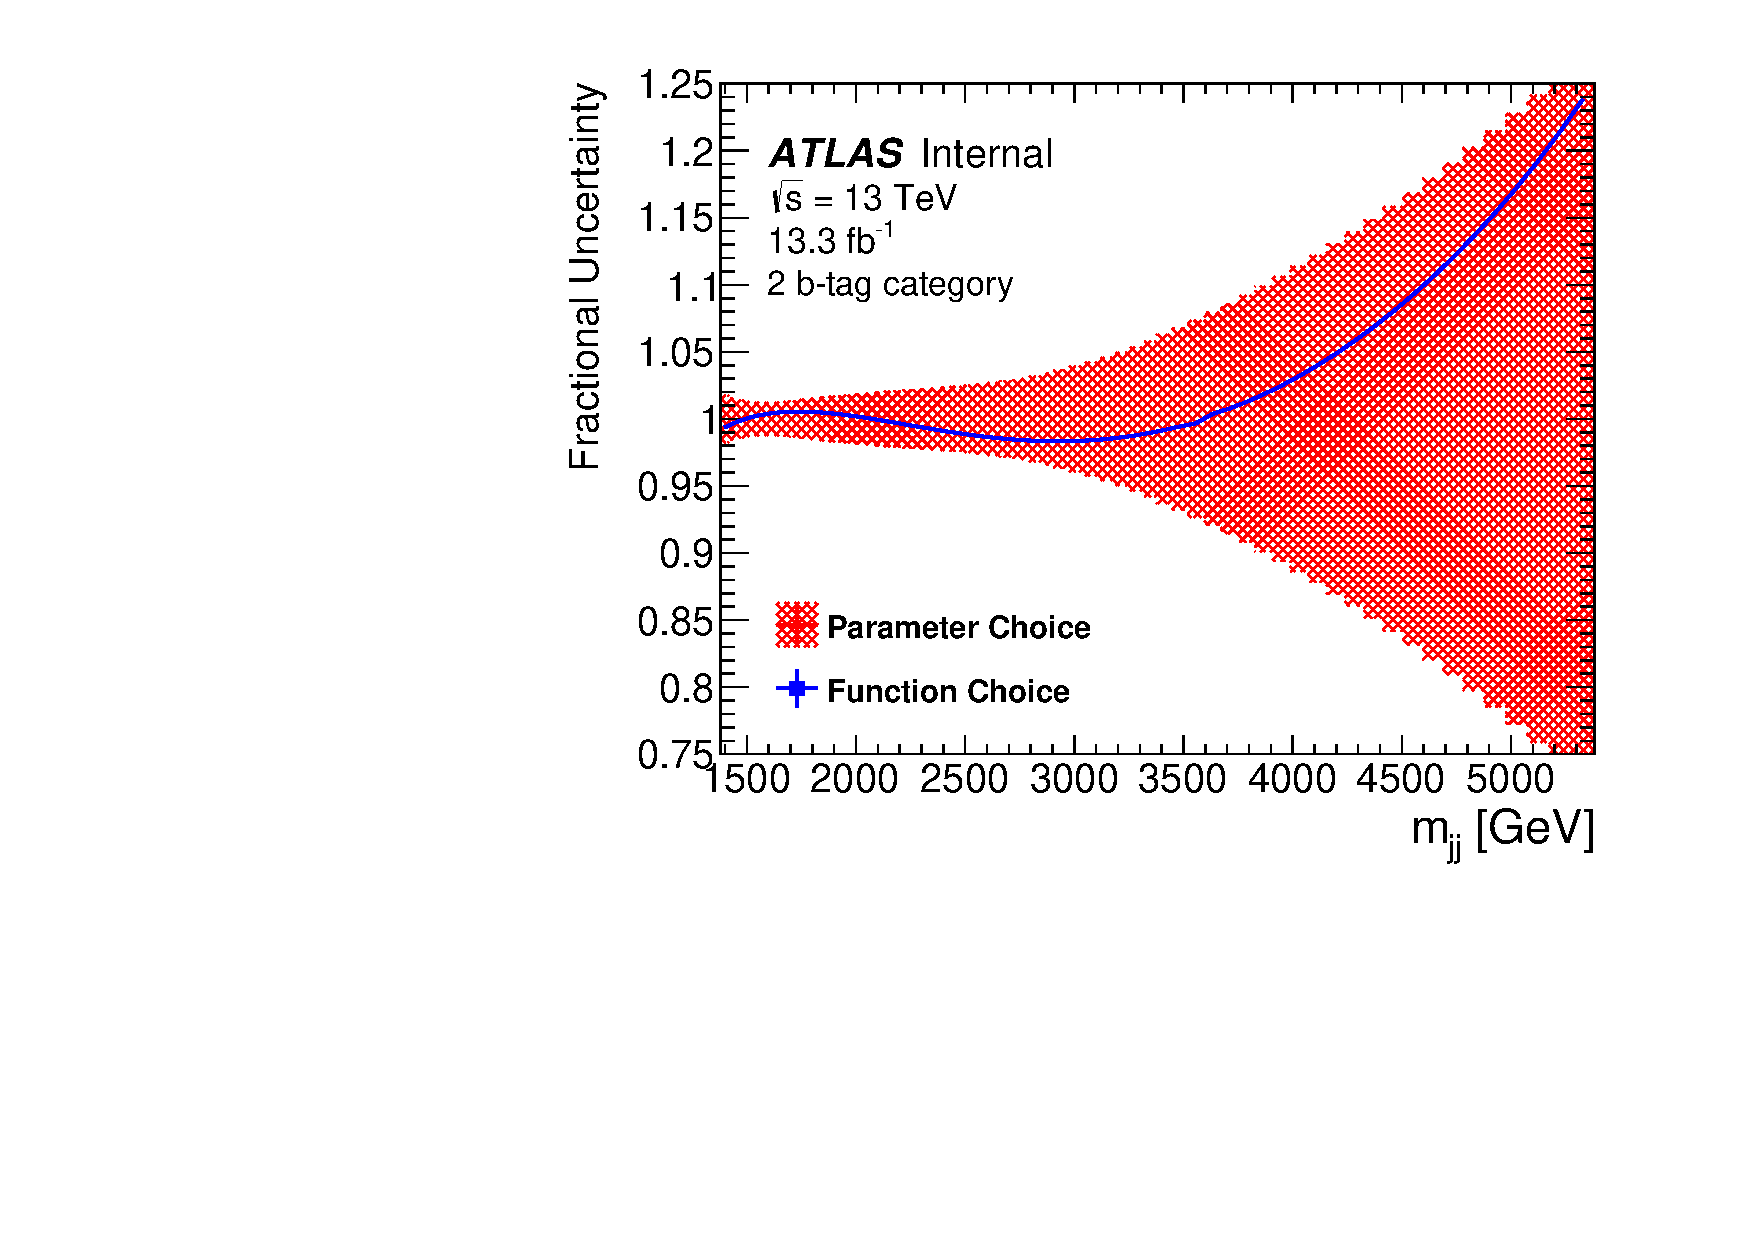
\includegraphics[width=0.47\linewidth, angle=0]{figs/Dibjet/ICHEP/lim-summer_systBkg_bb.pdf}}
    \subcaptionbox{$\geq$1 $b$-tag}{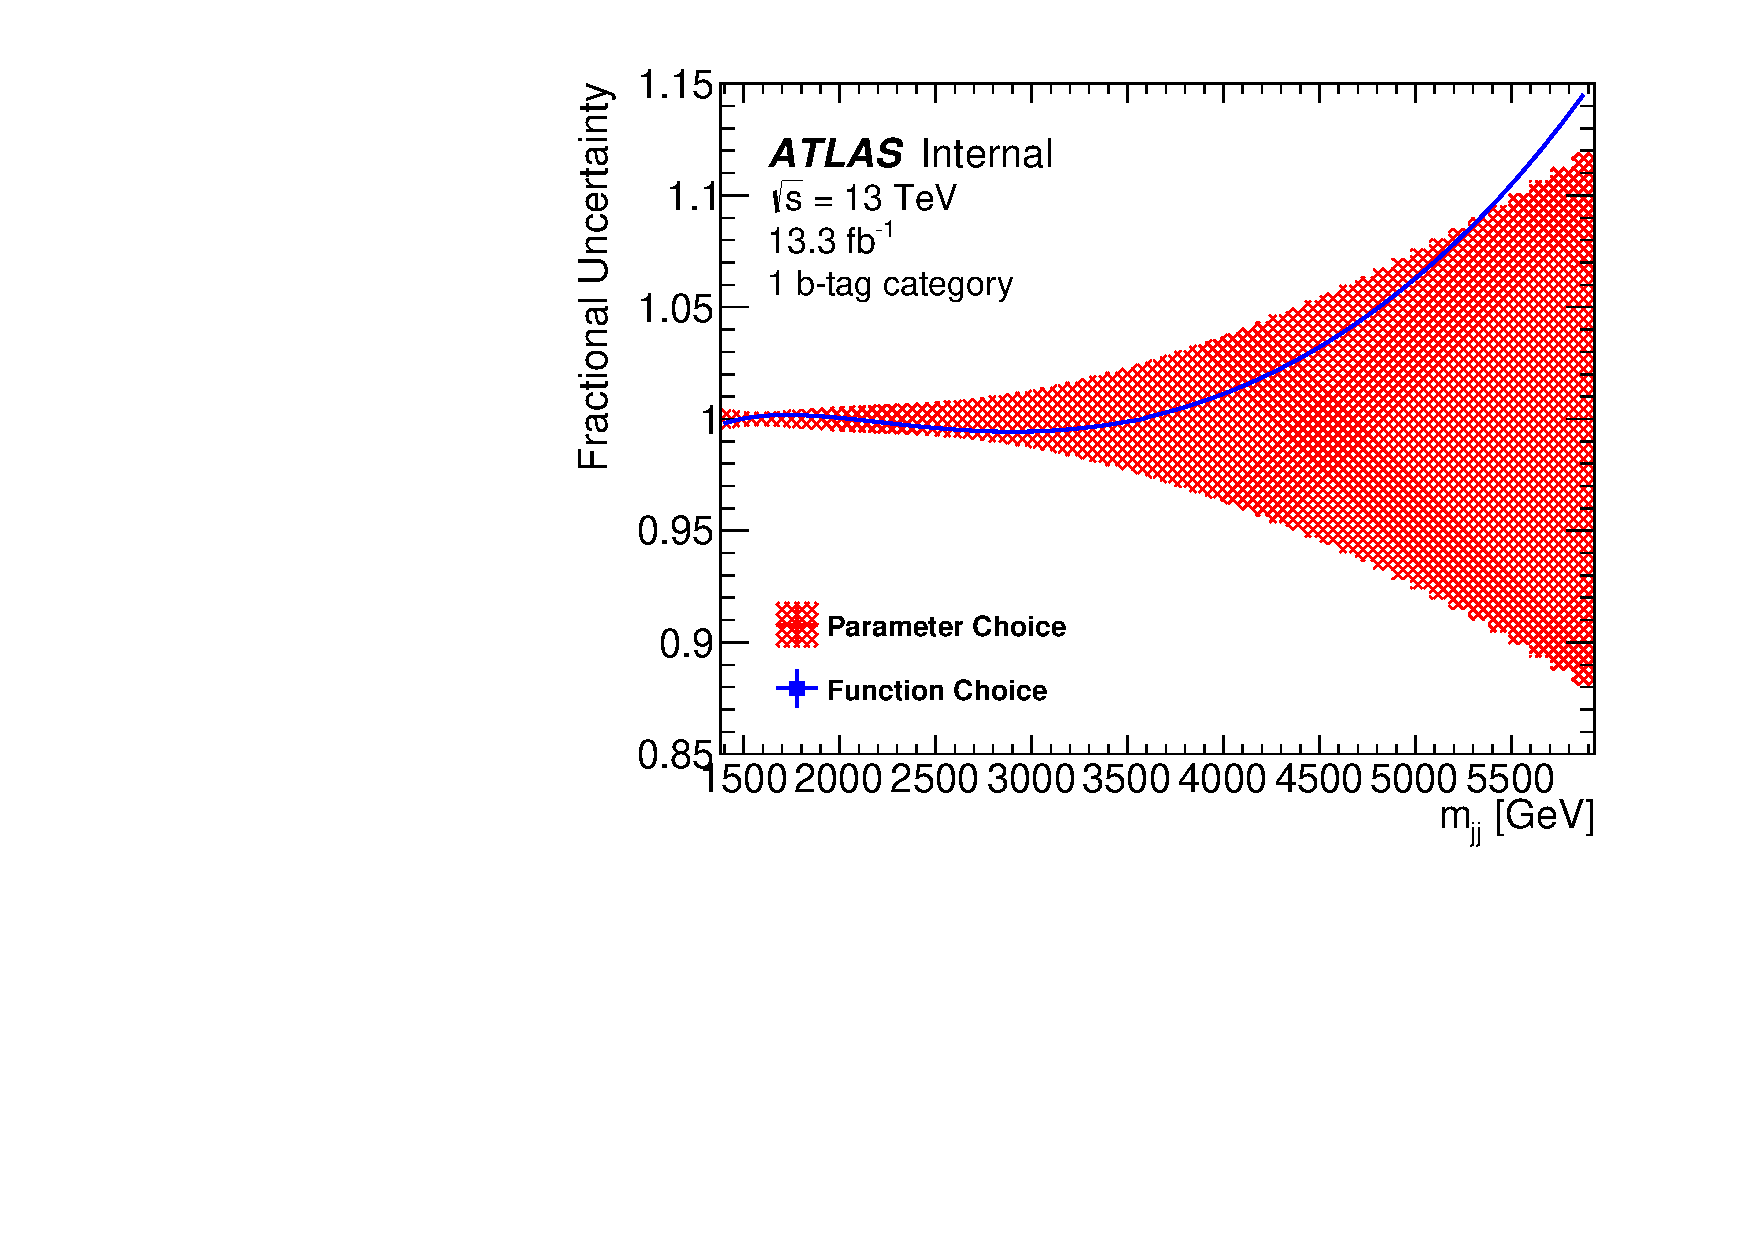
\includegraphics[width=0.47\linewidth, angle=0]{figs/Dibjet/ICHEP/lim-summer_systBkg_b.pdf}}
  \end{center}
  \vspace{-1em}
  \caption[The background systematic uncertainties as a function of dijet mass
    in the \summer{} data-set analysis.]
          {The fractional background systematic uncertainties for the (a) 2 and (b) $\geq$1 $b$-tag categories
            as a function of dijet mass,~\mjj, for the \summer{} data-set analysis.
            The red shaded region shows the function parameter uncertainty and
            the blue line shows the function choice uncertainty.  }
          \label{fig:lim-summer_systBkg}
\end{figure}

%Figure~\ref{fig:lim-summer_zprime} and \ref{fig:lim-summer_bstar} show the %% When there was two
Figure~\ref{fig:lim-summer_benchmark} shows the
95\% credibility level upper limits set on $\sigma\,\text{x}\,\mathit{A}\,\text{x}\,\epsilon$
as a function of generated mass
for the $Z'$ boson and $b^*$ quark.
%The signal models considered are described in Section~\ref{sec:evt-s+b}.
The observed limit, the expected limit and the associated 1 and 2 $\sigma$ uncertainty bands on the expected limit are shown.
The $\geq1$ $b$-tag category is used for the $b^*$ quark model
and the 2 $b$-tag category is used for the $Z'$ boson models.
%as these categories provide the strongest limits on the models.
Overlaid are theoretical predictions of
$\sigma\,\text{x}\,\mathit{A}\,\text{x}\,\epsilon$ for the benchmark models described in Section~\ref{sec:evt-s+b}.

%\begin{figure}[!ht]
%  \centering
%   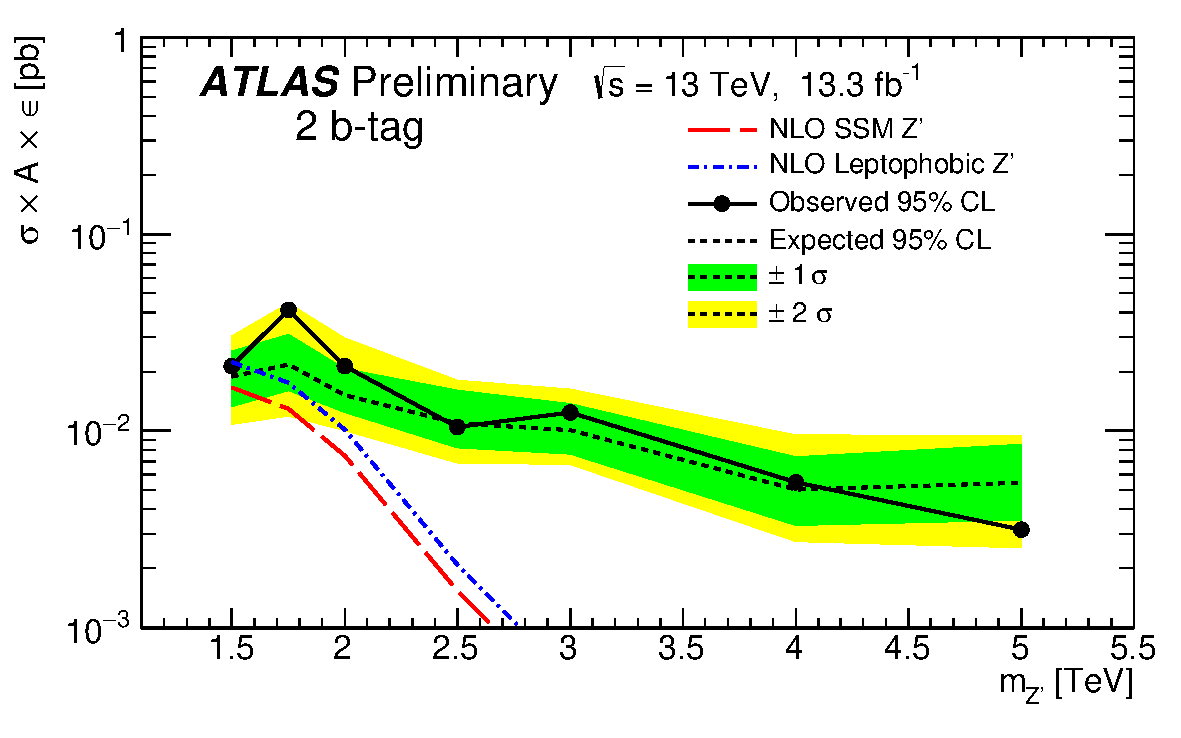
\includegraphics[width=0.7\linewidth, angle=0]{figs/Dibjet/ICHEP/lim-zprime.pdf}
%   \caption[Bayesian 95\% credibility level upper limits on cross-section times acceptance times tagging efficiency
%     for the $Z'$ boson as a function of generated mass
%     for the 2 $b$-tag category using the \summer{} data-set.
%     The observed limit is shown by the solid black line,
%     the expected limit is shown by the dotted black line
%     and the 1 and 2 $\sigma$ uncertainty bands are shown by the green and yellow bands respectively.
%     The theoretical predicition of $\sigma\,\text{x}\,\mathit{A}\,\text{x}\,\epsilon$
%     for the Sequential Standard Model (SSM) and leptophobic $Z'$ boson are overlaid.]
%           {Bayesian 95\% credibility level upper limits on cross-section times acceptance times tagging efficiency
%             for the $Z'$ boson as a function of generated mass
%             for the 2 $b$-tag category using the \summer{} data-set.
%             The observed limit is shown by the solid black line,
%             the expected limit is shown by the dotted black line
%             and the 1 and 2 $\sigma$ uncertainty bands are shown by the green and yellow bands respectively.
%             The theoretical predicitions of $\sigma\,\text{x}\,\mathit{A}\,\text{x}\,\epsilon$
%             for the Sequential Standard Model (SSM) and leptophobic $Z'$ boson are overlaid~\cite{dibjet-ichep_conf}.
%           }
%  \label{fig:lim-summer_zprime}
%  \vspace{1cm}
%  \centering
%   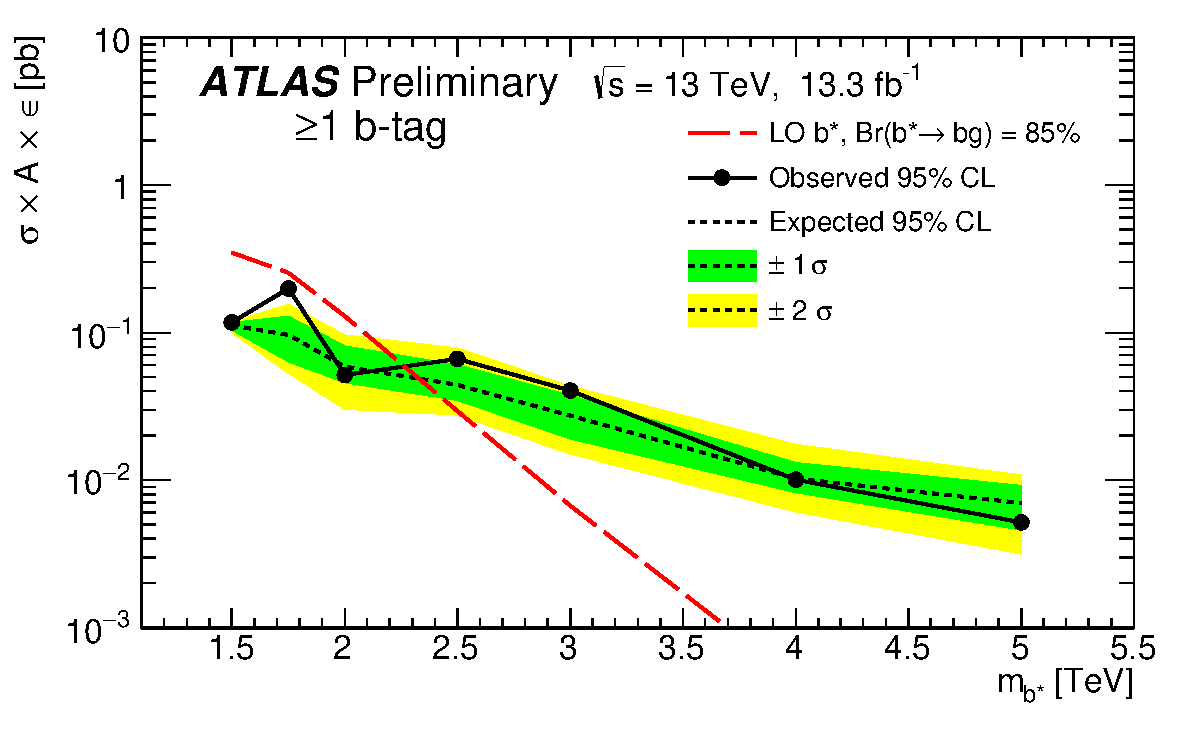
\includegraphics[width=0.7\linewidth, angle=0]{figs/Dibjet/ICHEP/lim-bstar.pdf}
%   \caption[Bayesian 95\% credibility level upper limits on cross-section times acceptance times tagging efficiency
%    for the $b^*$ quark  as a function of generated mass
%    for the $\geq$1 $b$-tag category using the \summer{} data-set.
%    The observed limit is shown by the solid black line,
%    the expected limit is shown by the dotted black line
%    and the 1 and 2 $\sigma$ uncertainty bands are shown by the green and yellow bands respectively.
%    The theoretical predicitions of $\sigma\,\text{x}\,\mathit{A}\,\text{x}\,\epsilon$
%    for the $b^*$ quark is overlaid.]
%           {Bayesian 95\% credibility level upper limits on cross-section times acceptance times tagging efficiency
%             for the $b^*$ quark  as a function of generated mass
%             for the $\geq$1 $b$-tag category using the \summer{} data-set.
%             The observed limit is shown by the solid black line,
%             the expected limit is shown by the dotted black line
%             and the 1 and 2 $\sigma$ uncertainty bands are shown by the green and yellow bands respectively.
%             The theoretical predicition of $\sigma\,\text{x}\,\mathit{A}\,\text{x}\,\epsilon$
%             for the $b^*$ quark is overlaid~\cite{dibjet-ichep_conf}.
%           }
%  \label{fig:lim-summer_bstar}
%\end{figure}


%The observed and expected limits decrease with increasing generated mass
%due to reduced number of background events at higher mass.
%The theoretical $\sigma\,\text{x}\,\mathit{A}\,\text{x}\,\epsilon$ predictions
%decrease rapidly as mass increases, due to a combination of
%lower signal acceptance times efficiency at high mass, as shown in Figures~\ref{fig:evt-ichep_acc},
%and a smaller signal cross-section at high mass.
%The signal cross-section is smaller at high mass because of PDF and matrix element effects,
%similar to those that caused a smaller QCD dijet production at high mass as described in
% Section~\ref{sec:theo-qcd-dijet_features}. 

In the mass regions where the theoretical prediction of $\sigma\,\text{x}\,\mathit{A}\,\text{x}\,\epsilon$
is larger than the upper limit, it can be concluded that the model is excluded at the 95\% credibility level.
Using the \summer{} data-set:
the \mbox{$b^*$ quark} is excluded in the mass range of 1.4~--~2.3~TeV,
the SSM $Z'$ boson cannot be excluded,
and the leptophobic $Z'$ boson is excluded at a mass of 1.5~TeV.

\begin{figure}[!htb]
  \centering
  \captionsetup[subfigure]{aboveskip=0pt,justification=centering}
  \subcaptionbox{$Z'$ boson,\hspace{1mm} 2 $b$-tag\vspace{12pt}}{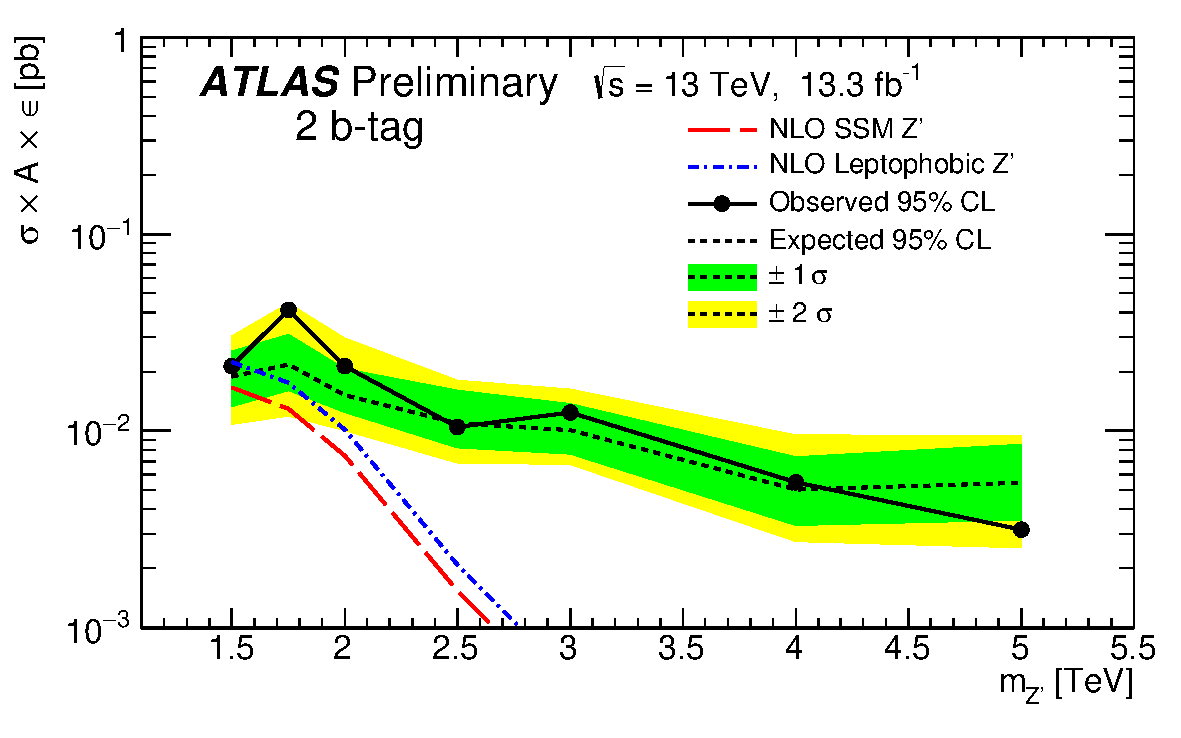
\includegraphics[width=0.9\linewidth, angle=0]{figs/Dibjet/ICHEP/lim-zprime.pdf}\vspace{-8pt}}
  \subcaptionbox{$b^*$ quark,\hspace{1mm} $\geq$1 $b$-tag}{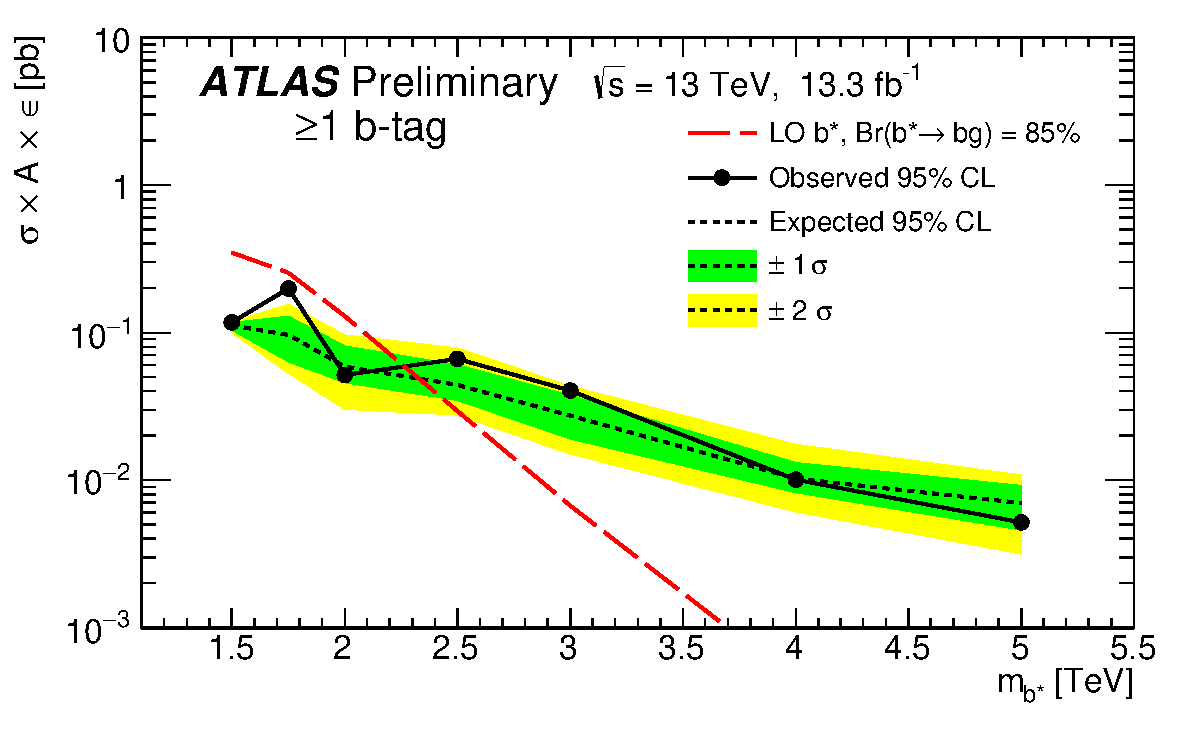
\includegraphics[width=0.9\linewidth, angle=0]{figs/Dibjet/ICHEP/lim-bstar.pdf}\vspace{-8pt}}
  \caption
      [95\% credibility level upper limits on the product of cross-section, detector acceptance and tagging efficiency
        for the $Z'$ boson and $b^*$ quark as a function of generated mass
        using the \summer{} data-set.]
      {95\% credibility level upper limits on
        the product of cross-section, detector acceptance and tagging efficiency ($\sigma\,\text{x}\,\mathit{A}\,\text{x}\,\epsilon$)
        for the (a) $Z'$ boson and (b) $b^*$ quark  as a function of generated mass
        using the \summer{} data-set in the 2 and $\geq$1 $b$-tag category respectively.
        The observed limit is shown by the solid black line,
        the expected limit is shown by the dotted black line,
        and the associated 1 and 2 $\sigma$ uncertainty bands on the expected limit are shown by the green and yellow bands.
        The theoretical predictions of $\sigma\,\text{x}\,\mathit{A}\,\text{x}\,\epsilon$
        for the Sequential Standard Model (SSM) and leptophobic $Z'$ boson and the $b^*$ quark are overlaid~\cite{dibjet-ichep_conf}.
      }
  \label{fig:lim-summer_benchmark}
\end{figure}

\newpage 
To produce generic Gaussian limits,
a signal template with a Gaussian shape in dijet mass is used.
The Gaussian distributions are centred on a range of mass points between 1.4 and 6.0~TeV,
the centre of the  Gaussian distribution is referred to as the generated mass.
The width of the Gaussian distributions are
15\%, 10\% and 7\% of the generated mass
in addition to a Gaussian with the width of the detector mass resolution.
The detector mass resolution has been estimated
at previous dijet searches~\cite{dijet-mori16_paper}
and varies from 3\% at 1.5~TeV to 2\% at~5~TeV.
%The dijet mass resolution is defined as the width of a Gaussian fit to mreco/mtruth
% for matched leading and subleading jets divided by the mean of the Gaussian.
The sources of the systematic uncertainty considered for the Gaussian limits 
are the luminosity uncertainty,
the background modelling uncertainties,
and a 10\% flat uncertainty to account for sources of
experimental uncertainties related to signal modelling,
such as jet energy scale.

Figure~\ref{fig:lim-summer_gauss} shows the observed 95\% credibility upper limits
on the product of cross-section, detector acceptance, tagging efficiency and branching ratio,
$\sigma\,\text{x}\,\mathit{A}\,\text{x}\,\epsilon\,\text{x}\,\mathit{BR}$,
for the full range of Gaussian signals described above in both $b$-tagging categories;
where the branching ratio is defined as the fraction of decays of the proposed BSM particle to 2 $b$-quarks in the 2 $b$-tag category,
or to a $b$-quark and a gluon in the $\geq1~b$-tag category.
For the \summer{} data-set analysis an upper limit is set on the $\sigma\,\text{x}\,\mathit{A}\,\text{x}\,\epsilon\,\text{x}\,\mathit{BR}$
for a generic Gaussian signal ranging from 0.2 to 0.001 pb in the mass range 1.4 to 6~TeV.

\begin{figure}[!ht]
  \begin{center}
    \captionsetup[subfigure]{aboveskip=0pt,justification=centering}
   \subcaptionbox{2 $b$-tag}      {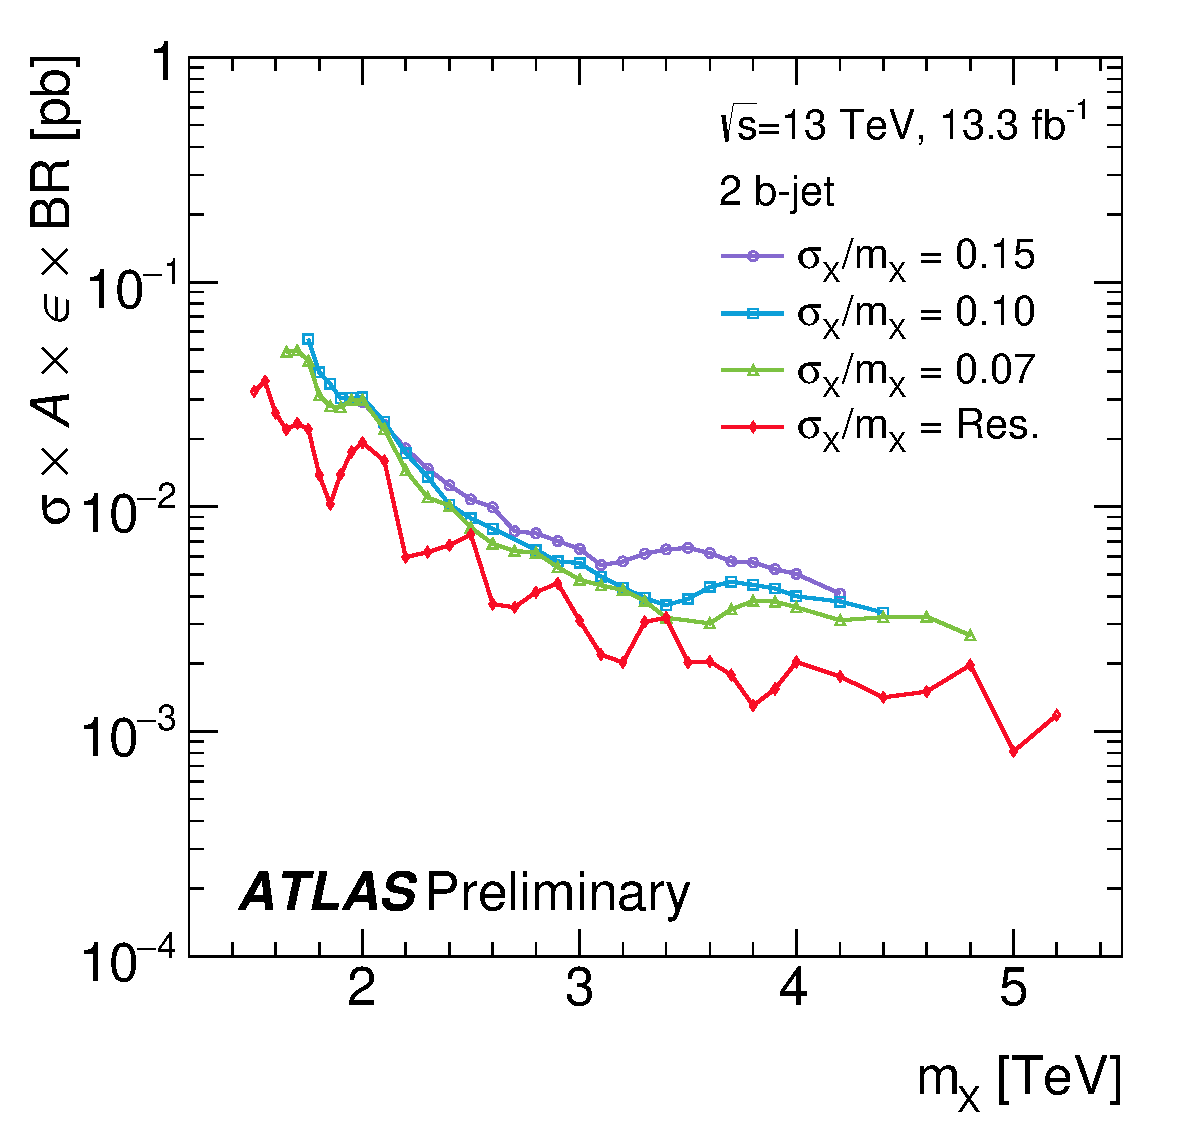
\includegraphics[width=0.49\linewidth, angle=0]{figs/Dibjet/ICHEP/lim-summer_gauss_bb.pdf}}
   \subcaptionbox{$\geq$1 $b$-tag}{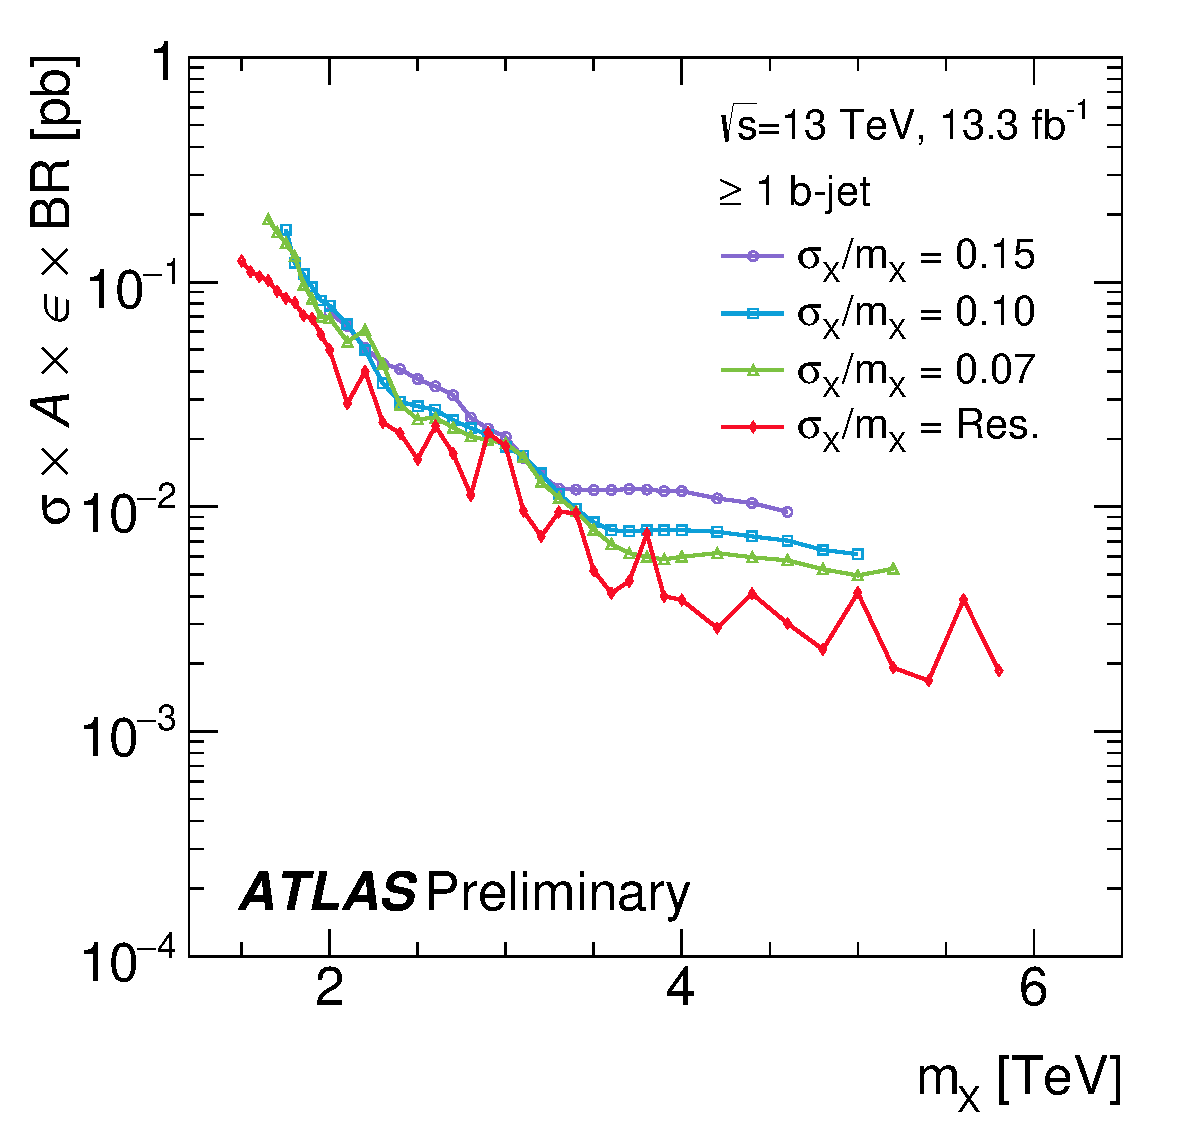
\includegraphics[width=0.49\linewidth, angle=0]{figs/Dibjet/ICHEP/lim-summer_gauss_b.pdf}}
  \end{center}
  \vspace{-1em}
  \caption[95\% credibility observed upper limits
    on the product of cross-section, detector acceptance, tagging efficiency and branching ratio
    for Gaussian signals using the \summer{} data-set.]
  {95\% credibility observed upper limits
    on the product of cross-section, detector acceptance, tagging efficiency and branching ratio,
    $\sigma\,\text{x}\,\mathit{A}\,\text{x}\,\epsilon\,\text{x}\,\mathit{BR}$,
    for Gaussian signals in both $b$-tagging categories using the \summer{} data-set.
    The signal templates are Gaussian in dijet  mass with
    widths of 15\%, 10\% and 7\% of the generated mass
    in addition to a Gaussian with the width of the detector mass resolution~\cite{dibjet-ichep_conf}.
  }
  \label{fig:lim-summer_gauss}
\end{figure}

\vfill
\clearpage

\section{\lm{} Data-set Limits}
\label{sec:lim-full}

\subsection{Signal Morphing}
\label{sec:lim-full_morphing}

The limit setting phase requires dijet mass signal templates as an input.
For the \lm{} data-set analysis, simulated dijet mass signal templates of the SSM $Z'$ boson are created at generated mass points of
600, 800, 1000 and 1250 GeV, as described in Section~\ref{sec:evt-s+b}.
To obtain dijet mass signal templates for intermediate points a signal morphing technique is used,
first implemented in an inclusive dijet search at ATLAS~\cite{dijet-mori17_paper}.

A `Gaussian + reverse Landau' fit is performed to the simulated dijet mass signal templates.
The reverse Landau function is the transformation of the Landau function~\cite{lim-landau} under $x\to-x$.
The Gaussian + reverse Landau fit function is therefore defined as:
\begin{equation}
  f(x)=p_0 \left[ \,p_1\,\mathrm{Gauss}\left(x,p_2,p_3\right)\,+\,\left(\,1-p_1\,\right)\,\mathrm{Landau}\,\left(-x,p_4,p_5\right)\, \right]
\end{equation}
The Gaussian distribution models the convolution of a Breit-Wigner resonance distribution and detector mass resolution effects.
The reverse Landau distribution provides a description of the off-shell contributions to the dijet mass signal templates which are enhanced at low mass by PDF effects.

\begin{figure}[!b]
  \vspace{-1.2em}
\begin{center}
  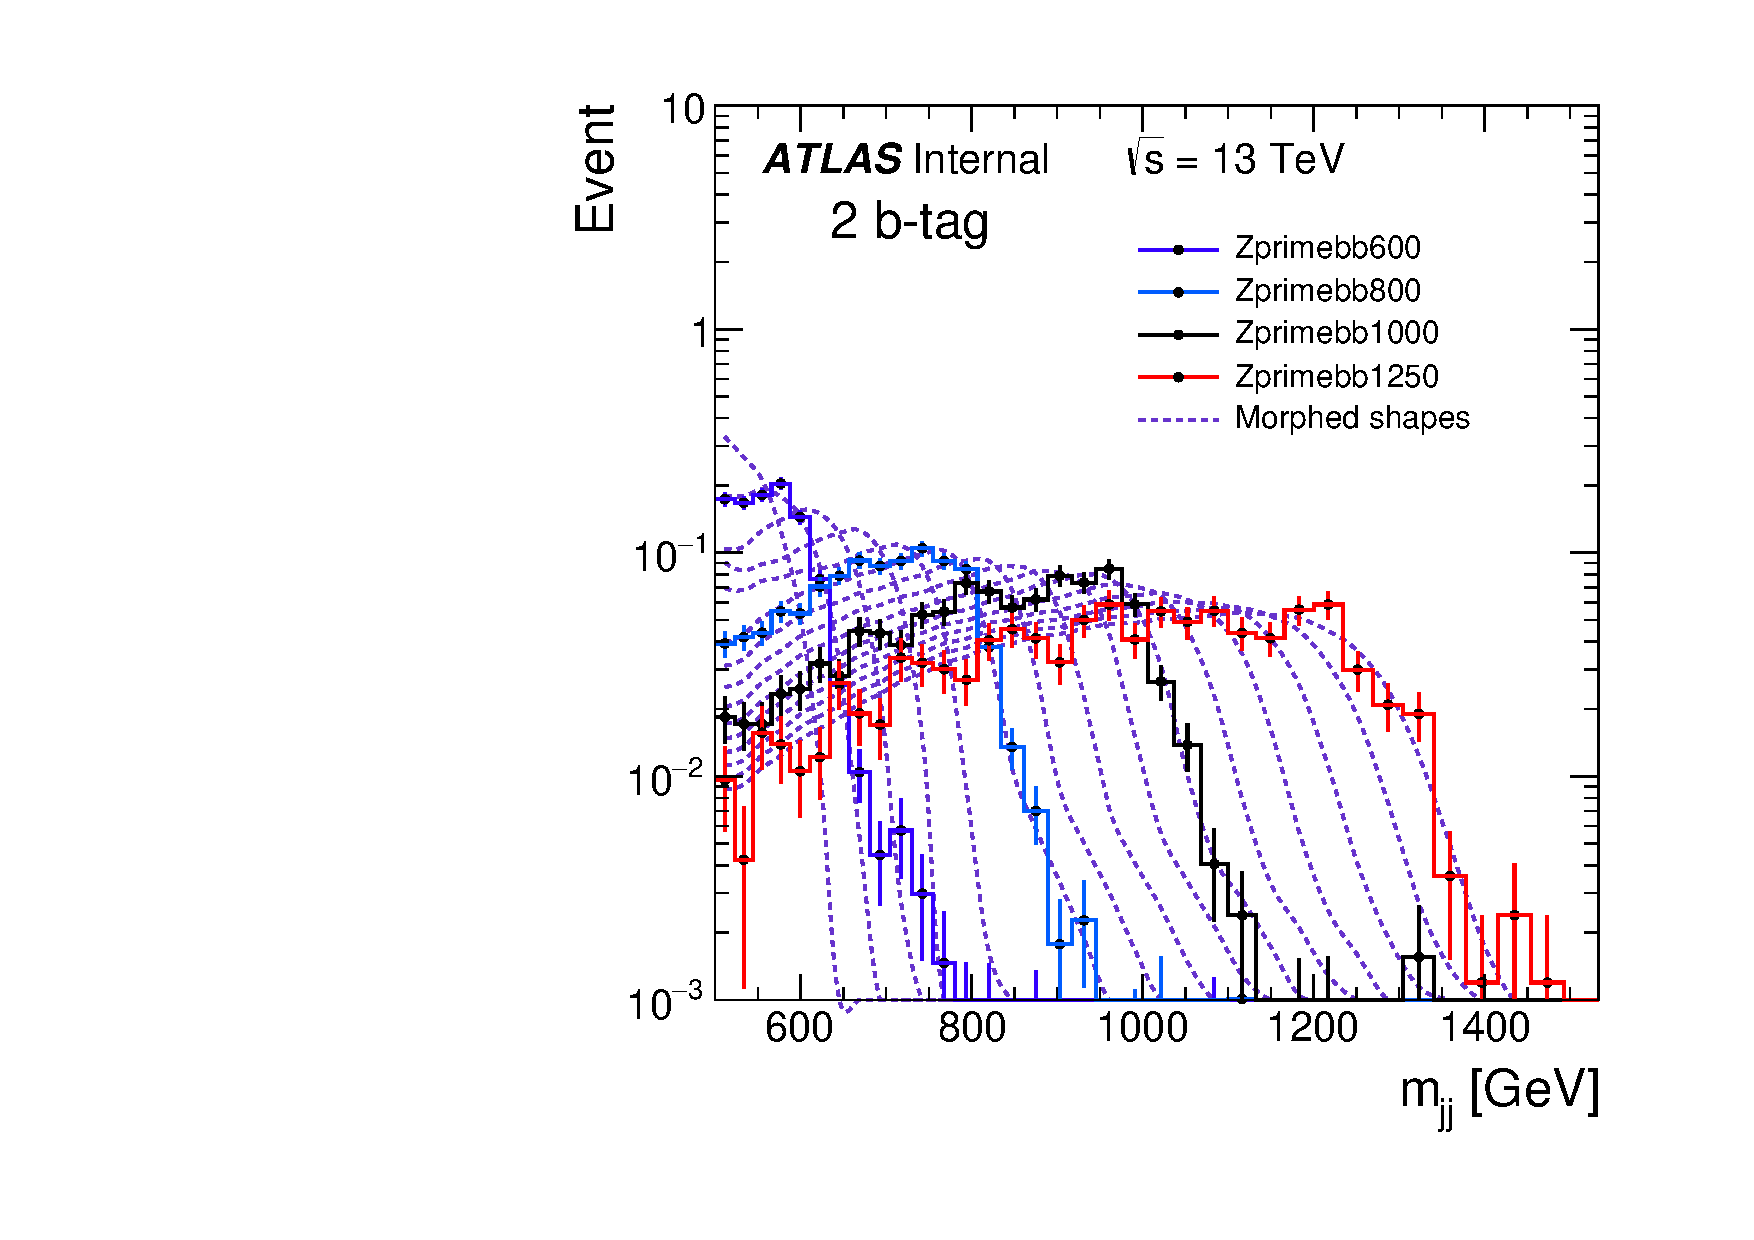
\includegraphics[width=0.47\linewidth, angle=0]{figs/Dibjet/LowMass/lim-morphing.pdf} 
\end{center}
\vspace{-2em}
\caption[Simulated SSM $Z'$ boson dijet mass signal templates and the intermediate dijet mass signal templates
  created using the signal morphing technique used in the \lm{} data-set limit setting phase.]
        {Simulated SSM $Z'$ boson dijet mass (\mjj) signal templates (solid points lines)
          at generated mass points of 600, 800, 1000 and 1250 GeV 
          and the dijet mass signal templates created using the signal morphing technique (dotted lines). The \lm{} event selection has been applied~\cite{dibjet-full_int}.
          \label{fig:lim-full_morphing}}
\end{figure}

The parameters of the Gaussian + reverse Landau fits are interpolated to produce dijet mass signal templates at intermediary generated mass points
in the range 600 to 1250 GeV with a separation of 50 GeV \footnote{\ Explicitly morphed signal templates are created at generated mass points of 650, 700, 750, 850, 900, 950, 1050, 1100, 1150 and 1200 GeV.}.
Figure~\ref{fig:lim-full_morphing} shows the simulated SSM $Z'$ boson dijet mass signal templates and the intermediate dijet mass signal templates produced using the morphing procedure.
The simulated and morphed signal dijet mass spectra are used as signal templates in the limit setting phase for the \lm{} data-set analysis.


\subsection{Summary of Systematic Uncertainties}
\label{sec:lim-full_systs}

Table~\ref{tab:lim-lowmass_syst} summarises the systematic uncertainties considered for the
signal templates used in the \lm{} data-set at three different dijet masses.
Figure~\ref{fig:lim-lowmass_syst}(a) shows the total $b$-jet trigger systematic uncertainty as a function of dijet  mass;
this includes both the jet-level and event-level uncertainties described in Section~\ref{sec:trig-bjet_eff}.
Figure~\ref{fig:lim-lowmass_syst}(b) shows the systematic uncertainties on the background estimate as a function of dijet  mass.
%Reconstructed mass is defined as invariant mass of the two observed jets.
%$b$-tagging, $b$-jet trigger and $b$-jet energy scale are the dominant sources of systematic uncertainties at the lowest mass point,
%whilst for the remaining dijet mass range $b$-jet trigger uncertainties are dominant.

\begin{table}[!htb]
  \centering
  \begin{tabular}{|c||c|c|c|c|c|c|c|}
    \hline
    \textbf{Dijet}   & \multicolumn{7}{c|}{\textbf{Signal Systematic Uncertainties}}                    \\ \cline{2-8} 
    \textbf{Mass}    & JES   & JER   & $b$JES  & $b$-Tagging & $b$-Jet Trigger & PDF & Lumi.        \\
    \hline                                                                        
    0.6~TeV          & 0.9\% & 1.4\% & 5\%     &     5\%     &      5.4\%   & 1\% & 2.2\%       \\
    1.0~TeV          & 0.8\% & 1.2\% & 3\%     &     7\%     &       15\%   & 1\% & 2.2\%       \\
    1.5~TeV          & 1.1\% & 1.0\% & 1.8\%    &    10\%     &       29\%   & 1\% & 2.2\%       \\
    \hline
    % The background uncertainties
    %& \multicolumn{2}{c|}{Bkg. Uncert}             
    %&  Para. ($\geq$1 / 2)   & Func. ($\geq$1 / 2) 
    %                                               
    %&  1.3\%/0.0\%      & 0.3\%/0.0\%              
    %&  3.9\%/1.7\%      & 1.3\%/0.6\%           
    %&   22\%/ 17\%      & 7.5\%/5.1\%
  \end{tabular}
  \caption[The signal systematic uncertainties used in the \lm{} data-set analysis.]
          {The signal systematic uncertainties used in the \lm{} data-set analysis
           for three different dijet mass (\mjj{}) points.
          Jet Energy Scale (JES), Jet Energy Resolution (JER) and $b$-jet Energy Scale ($b$JES)
          are uncertainties on the dijet mass of a simulated event,
          whilst $b$-tagging, $b$-jet trigger, PDF and luminosity uncertainties are uncertainties on simulated event weight.
          All values except the $b$-jet trigger uncertainty are taken from~\cite{dibjet-full_int}.}
  \label{tab:lim-lowmass_syst}
  \end{table}

\begin{figure}[!ht]
  \begin{center}
    \captionsetup[subfigure]{aboveskip=0pt,justification=centering}
    \subcaptionbox{$b$-Jet Trigger Uncertainty}{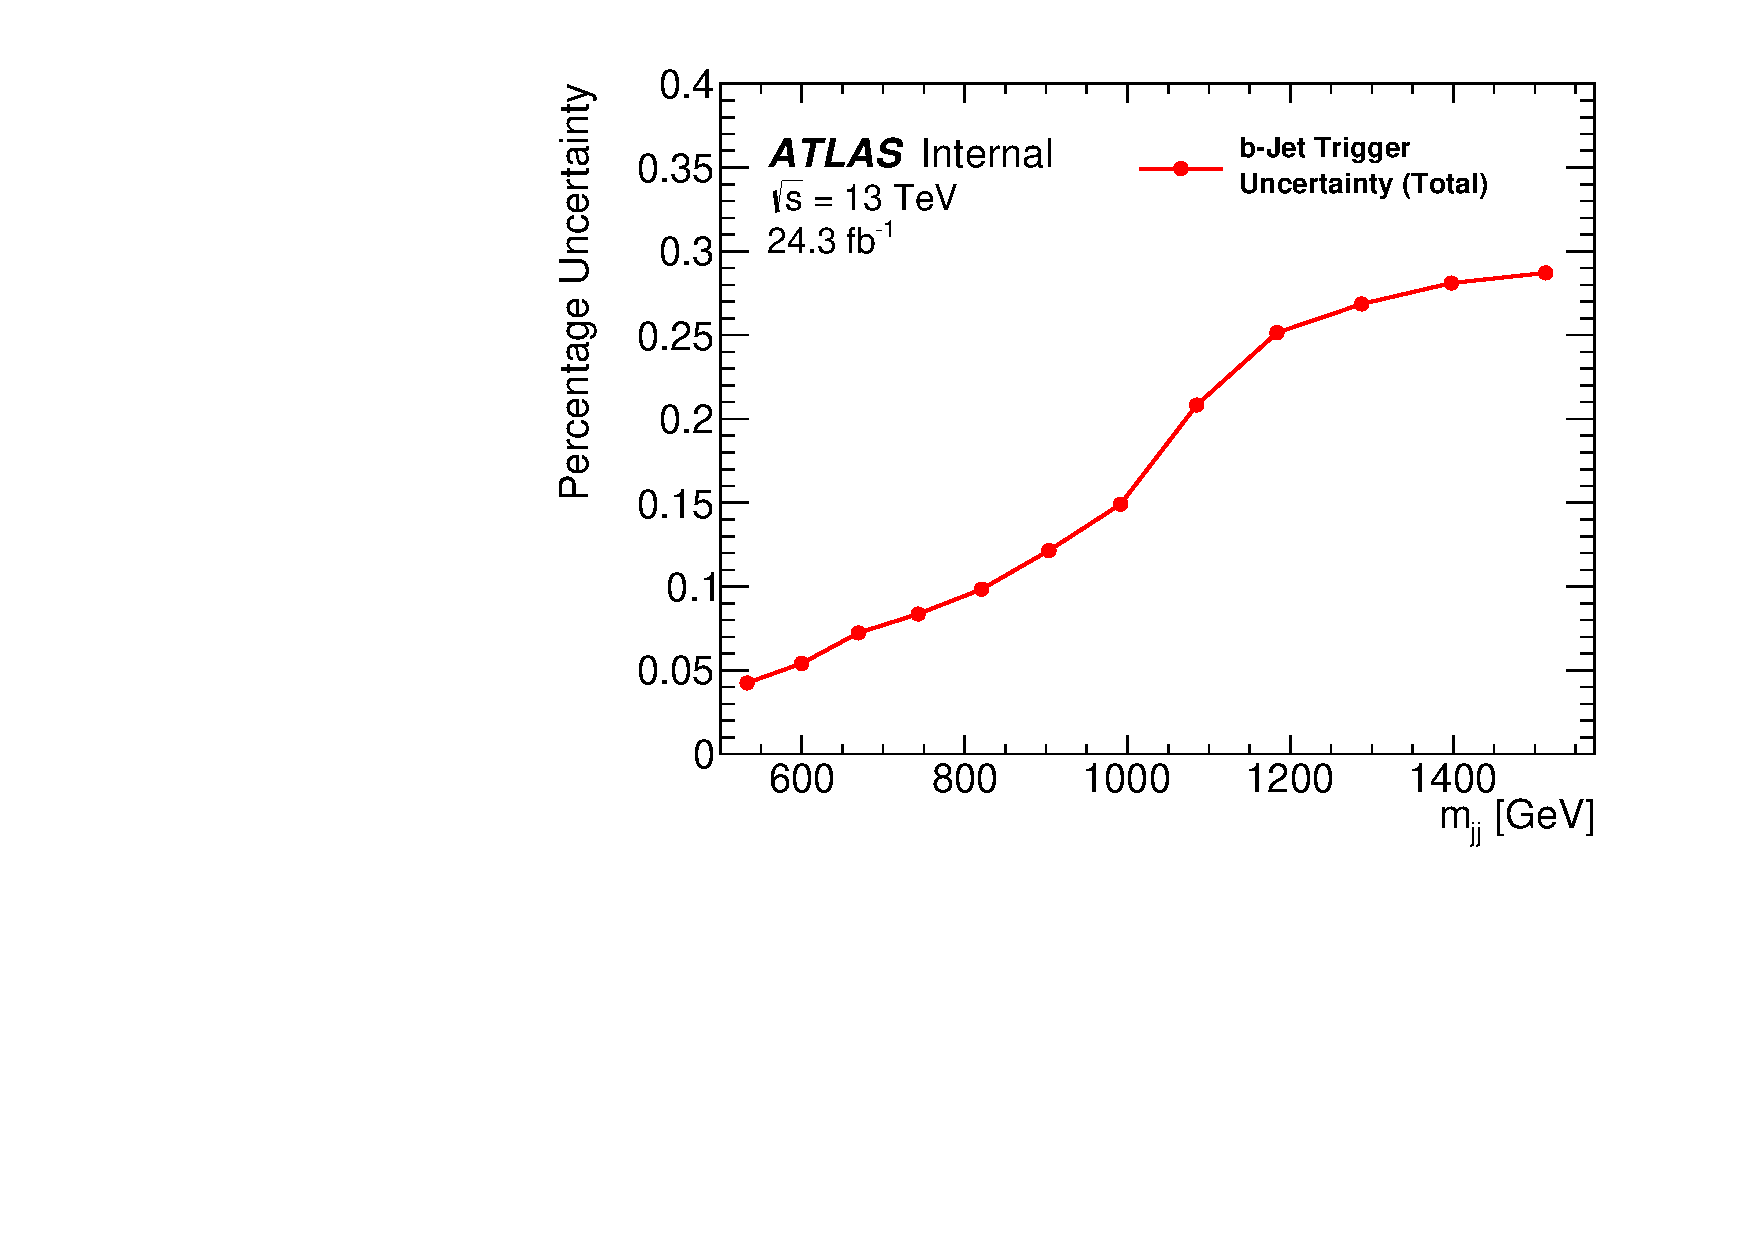
\includegraphics[width=0.47\linewidth, angle=0]{figs/Dibjet/LowMass/lim-bTrigUncert.pdf}}
    \subcaptionbox{Background Uncertainties}{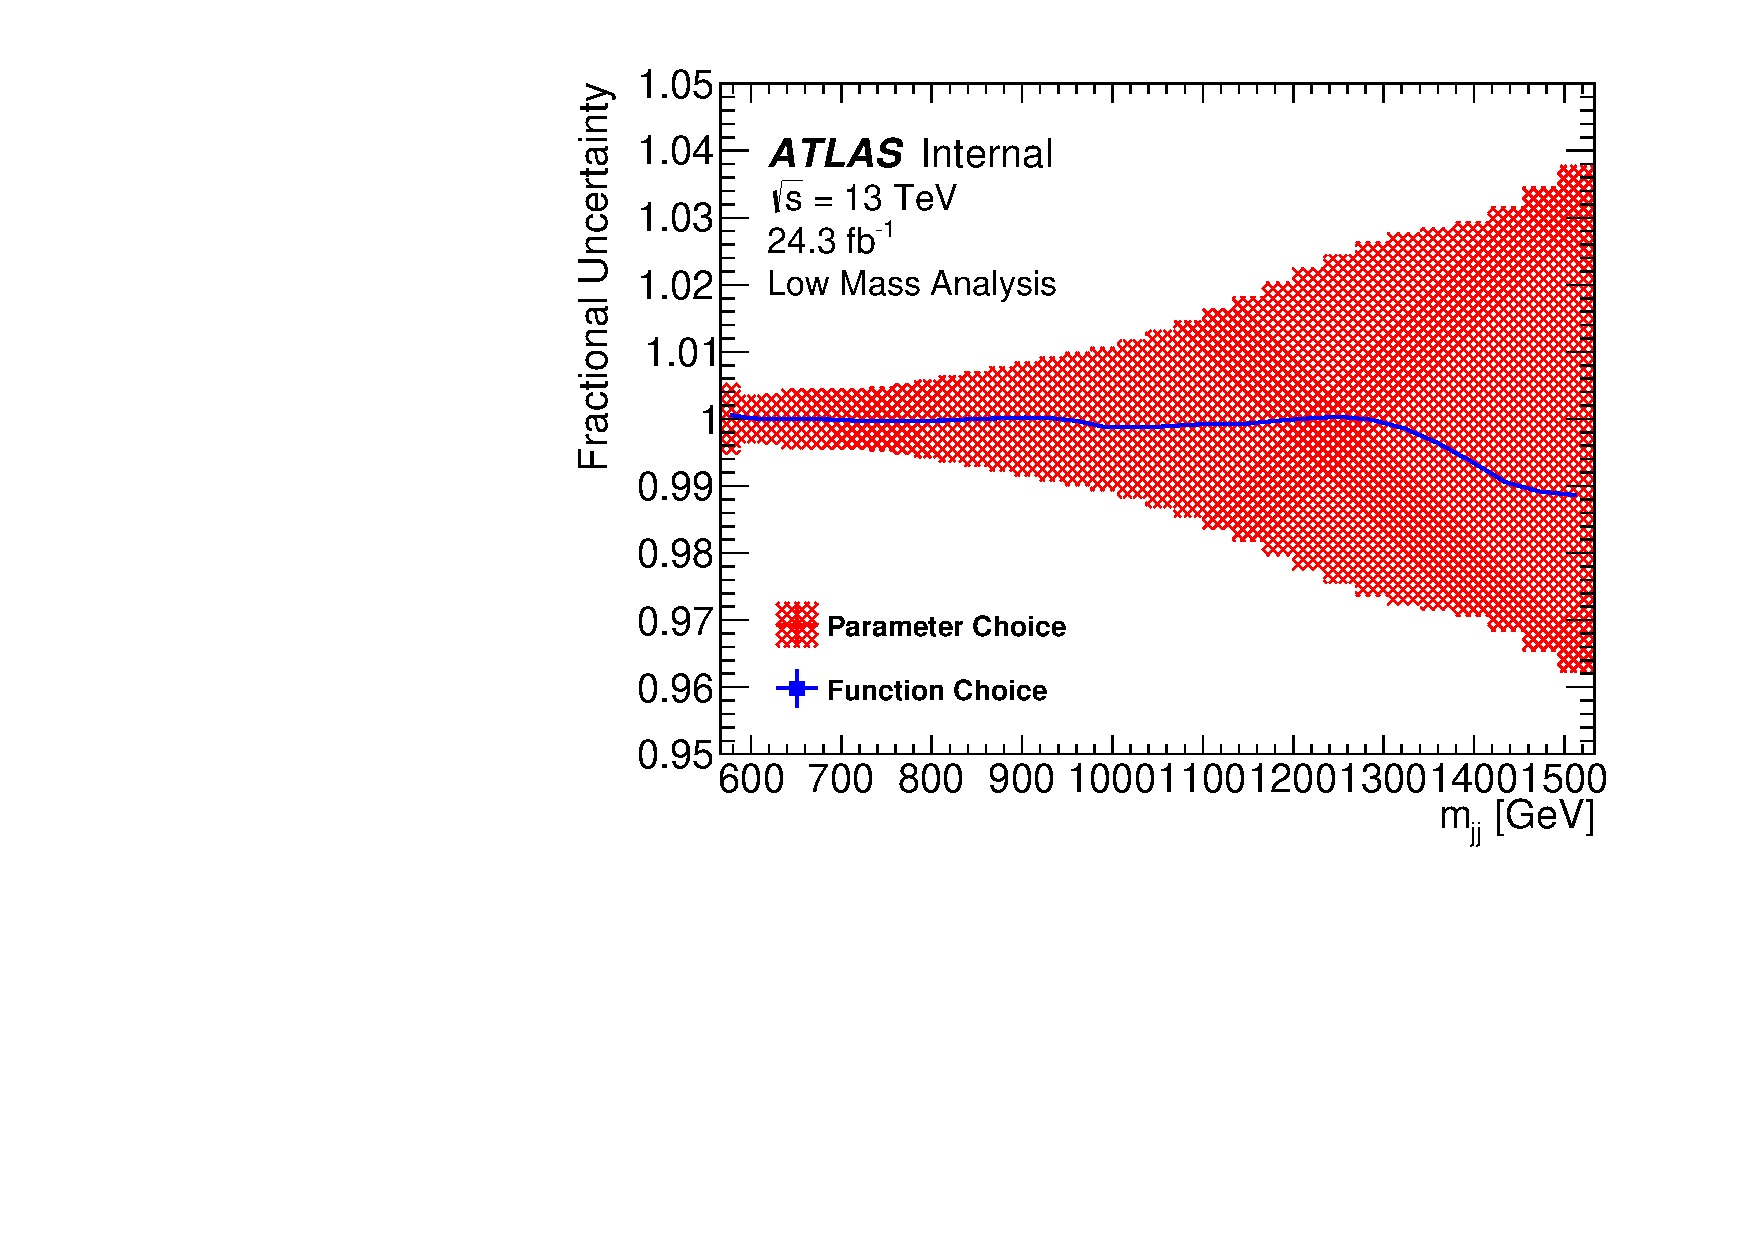
\includegraphics[width=0.47\linewidth, angle=0]{figs/Dibjet/LowMass/lim-lowmass_systBkg.pdf}}
  \end{center}
  \vspace{-1em}
  \caption[The $b$-jet trigger and background systematic uncertainties for the \lm{} data-set as a function of dijet mass.]
    {Panel (a) shows the total $b$-jet trigger systematic uncertainty as a fraction for the \lm{} data-set as a function of dijet mass (\mjj).
    Panel (b) shows the background systematic uncertainties as a fraction for the \lm{} data-set as a function of dijet mass;
    the red shaded region shows the function parameter uncertainty and the blue line shows the function choice uncertainty.}
  \label{fig:lim-lowmass_syst}
\end{figure}

\subsection{Signal Subtracted Background Estimation}
\label{sec:lim-full_ssb}

Section~\ref{sec:bkg-full_swift} described the SWiFt background estimation procedure used in the search phase of the \lm{} data-set, 
for clarity this will be referred to as the \textit{`nominal SWiFt background estimation'} in this section.
The nominal SWiFt background estimation is model independent as there is no assumption of any signal models in the procedure.
In Section~\ref{sec:bkg-full_signalInj} it was shown that there is a signal induced fit bias present when
the nominal SWiFt background estimation is performed on a background-only test data-set with a SSM $Z'$ boson injected.
This is particularly notable for a SSM $Z'$ boson with a generated mass of 600~GeV,
as this is near the edge of the dijet mass spectrum considered.

To remove any signal induced fit bias in the limit setting phase, a signal plus background fit
is performed for each signal point considered in the limit setting phase.
The signal is modelled using the dijet mass signal templates described in Section~\ref{sec:lim-full_morphing}
and the background is modelled using the 5 parameter dijet fit function.
The signal plus background fit is performed in the SWiFt window in which the generated mass of the signal being considered is at the window centre,
the fit does not use the full mass range as it has been shown in Section~\ref{sec:bkg-full_globalFit} that a global background fit is not reliable.
A window half-width of 16 and the 5 parameter dijet fit function are chosen to match the configuration used in the search phase results shown in Section~\ref{sec:bkg-full_results}.
The normalisation of the signal template and the parameters of the background fit function are
chosen to maximise the likelihood (defined in Equation~\ref{eqn:lim-like}), the signal normalisation is required to be greater or equal to zero.

The signal plus background fit provides an estimate of the number of signal and background events in the SWiFt window considered,
however the framework used for the limit setting phase requires a background estimation for the full mass range considered.
To extend the background estimate to the full range, the signal template, normalised by the signal plus background fit, is subtracted from the data.
The SWiFt background estimation procedure is then performed to the signal subtracted data,
using the 5 parameter dijet fit function and a window half-width of 16, which is again chosen to match the configuration used in the search phase.
The resulting background estimation is known as the \textit{`signal subtracted background estimation'} (SSB).
A signal subtracted background estimation is created for each generated mass point and
is used as the background template in the limit setting phase for the \lm{} data-set analysis.

The signal subtracted background estimate is used as it provides a simple method of using the results of the signal plus background fit
performed in a SWiFt window to create a background estimate for the full mass range. 
Furthermore, the signal subtracted background estimate is used by the most recent inclusive dijet search at ATLAS~\cite{dijet-mori17_paper}.
It is beneficial for related analyses at ATLAS to utilise similar background estimation techniques for three main reasons:
it increases reliability as the technique is independently validated multiple times,
shares framework development responsibilities between multiple analyses,
%increases the productivity of ATLAS due to the sharing of computing framework,
and leads to greater consistency in the presentation of ATLAS results.

To demonstrate that the signal subtracted background estimation will remove the signal induced fit bias,
the procedure is performed to a data-like dijet mass spectrum from the fit control region when a SSM $Z'$ boson dijet mass signal template is injected.
The same distributions were used in the signal injection studies presented in Section~\ref{sec:bkg-full_signalInj}.
The performance of the signal subtracted background estimation can be compared to that of the nominal SWiFt background estimation.

In Figure~\ref{fig:lim-lowmass_ssb_test}(a) the nominal SWiFt background estimate~(red) and the signal subtracted background estimate~(blue)
for a data-like dijet mass spectrum from the fit control region with a SSM $Z'$ boson injected at 600 GeV are
shown as a ratio to the nominal SWiFt background estimation for the same data-like dijet mass spectrum when no signal is injected (black).
This ratio is used to clearly show any signal induced fit biases.
The signal injected dijet mass spectrum is shown by the green points and the grey area represents the statistical uncertainty of the data.
Figure~\ref{fig:lim-lowmass_ssb_test}(b) shows the same comparison using a SSM $Z'$ boson injected at 1000 GeV.
These two mass points are shown as the signal injection studies, presented in Section~\ref{sec:bkg-full_signalInj},
found that the search phase would not produce a significant observation of a SSM $Z'$ boson at these generated mass points. 

\begin{figure}[!ht]
  \begin{center}
    \captionsetup[subfigure]{aboveskip=0pt,justification=centering}
    \subcaptionbox{$Z'$ boson, $m$ = 600 GeV}{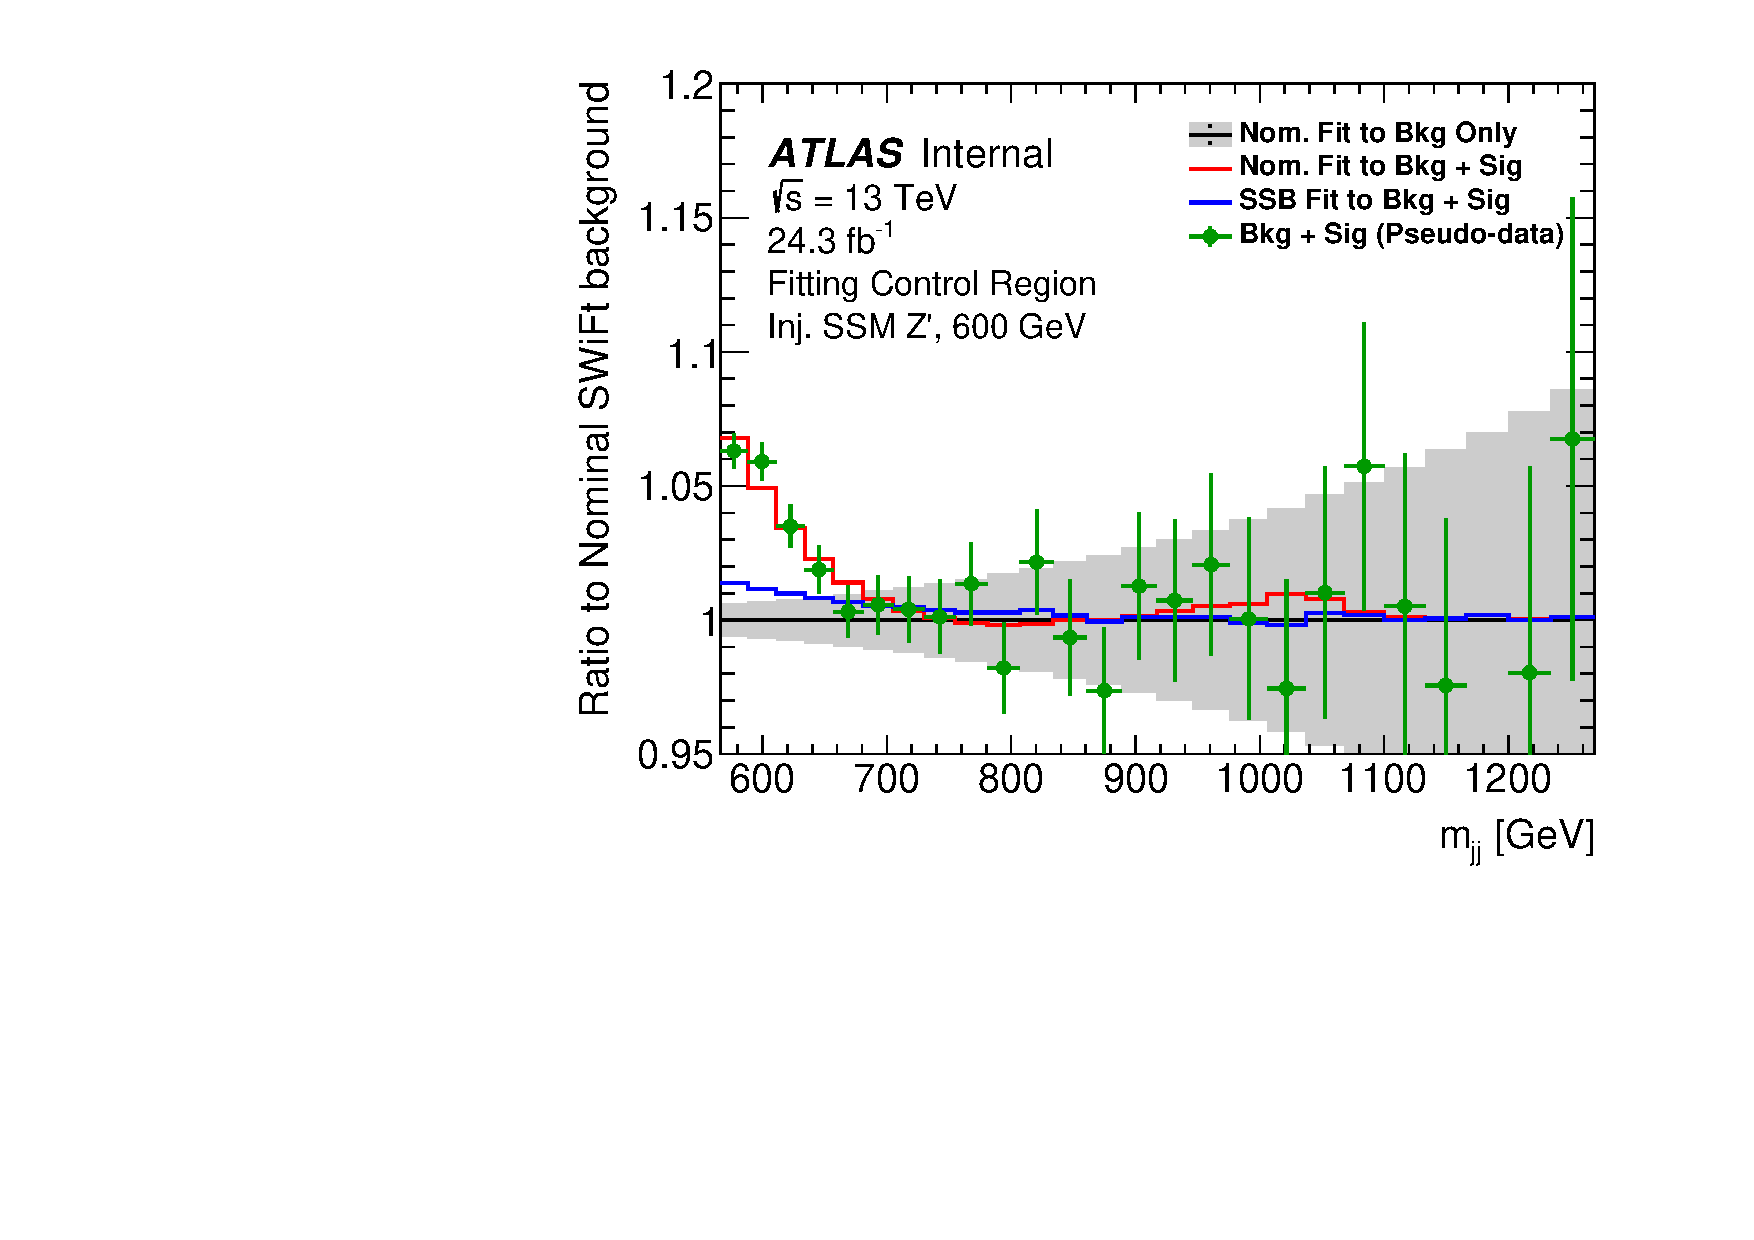
\includegraphics[width=0.51\linewidth, angle=0]{figs/Dibjet/LowMass/lim-ssb_test600.pdf}} \hspace{-7mm}
    \subcaptionbox{$Z'$ boson, $m$ = 1000 GeV}{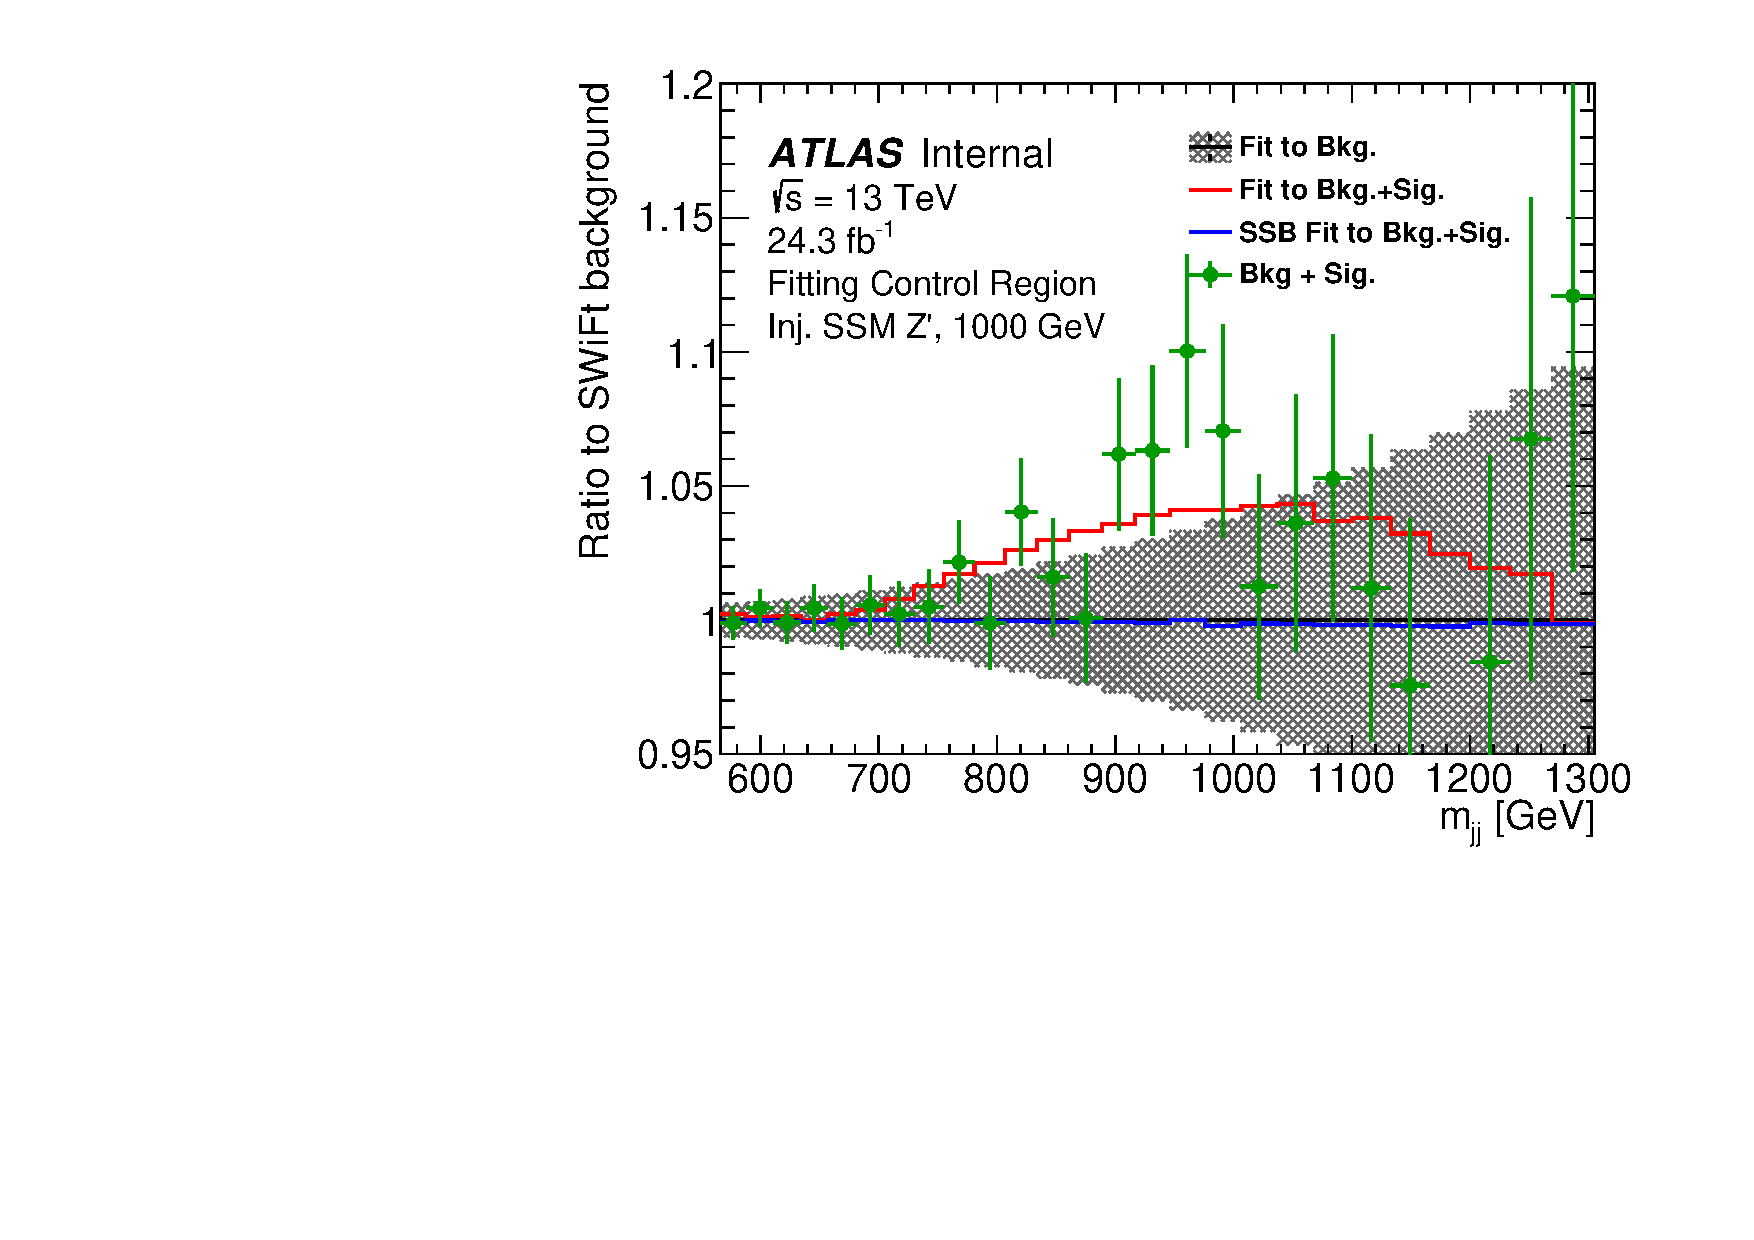
\includegraphics[width=0.51\linewidth, angle=0]{figs/Dibjet/LowMass/lim-ssb_test1000.pdf}} \hspace{-5mm}
  \end{center}
  \vspace{-1em}
  \caption[The nominal SWiFt background and signal subtracted background estimations
    for a data-like dijet mass  spectrum from the fit control region with a SSM $Z'$ boson injected
    as a ratio to the nominal SWiFt background estimation performed on the same data-like dijet mass spectrum when no signal is injected.]
          {The nominal SWiFt background (red) and signal subtracted background (SSB) (blue) estimations
    for a data-like dijet mass (\mjj) spectrum from the fit control region with a SSM $Z'$ boson injected (green points)
    as a ratio to the nominal SWiFt background estimation performed on the same data-like dijet mass spectrum when no signal is injected.
    The grey area represents the statistical uncertainties of the data-set.
    The generated mass of the SSM $Z'$ boson is (a) 600 GeV and (b) 1000 GeV.
    The nominal SWiFt background estimation procedure is used in the search phase,
          the signal subtracted background estimation procedure is used in the limit setting phase.}
  \label{fig:lim-lowmass_ssb_test}
\end{figure}

The nominal SWiFt background estimation has a large signal induced fit bias when a SSM $Z'$ boson is injected,
shown by the fact that the red line is significantly drawn towards the injected signal in Figure~\ref{fig:lim-lowmass_ssb_test}.
The signal induced fit bias is especially notable in the case of a SSM $Z'$ boson at 600 GeV.
The signal induced fit bias of the signal subtracted background is small relative to the size of the injected signal,
shown by the fact that the blue line lies close to one for all dijet masses.
Therefore, the signal subtracted background estimation is used in the limit setting phase of the \lm{} data-set analysis,
for both the $Z'$ boson and generic Gaussian signals.
A signal subtracted background estimate is created for each signal mass point using the dijet mass spectrum observed in data.

If the signal subtracted background estimates differ greatly from the nominal SWiFt background estimate,
this is evidence that there may be a signal induced fit bias present in the search phase.
Figure~\ref{fig:lim-lowmass_ssb_data} shows the ratio of the 
signal subtracted background estimations to the nominal SWiFt background estimate (black) performed on the full \lm{} data-set
\footnote{\ The SWiFt background estimate for the full data-set is shown in comparison to the data in Figure~\ref{fig:bhFit_lm_unblind}.}.
The grey area represents the parameter choice uncertainty of the nominal SWiFt background estimation.
Signal subtracted background estimations are created for all generated mass points considered,
but for clarity only those at mass points of 600, 800, 1000 and 1250~GeV are shown in the figure.

\begin{figure}[!htb]
  \begin{center}
    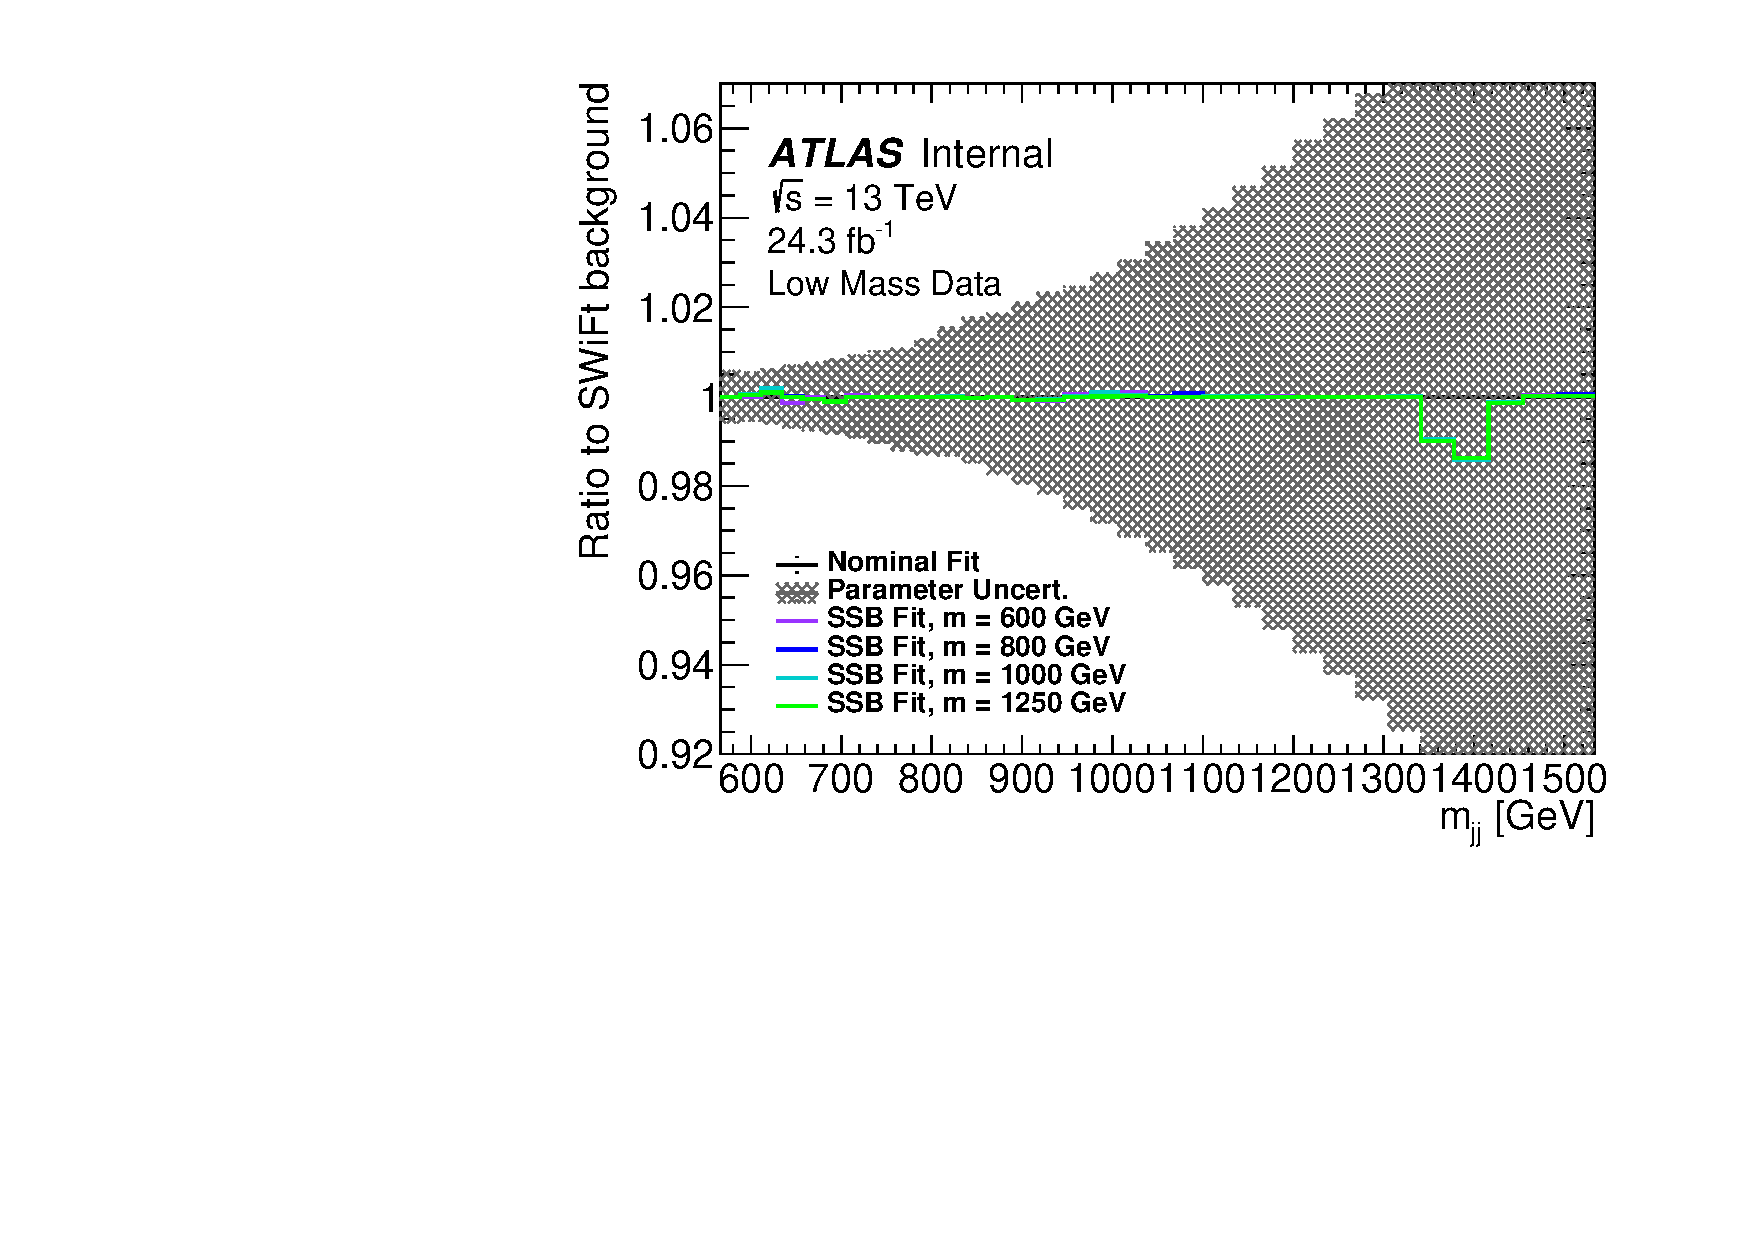
\includegraphics[width=0.6\linewidth, angle=0]{figs/Dibjet/LowMass/lim-ssb_data.pdf}
  \end{center}
  \vspace{-1em}
  \caption[The ratio of signal subtracted background estimations
    and the SWiFt background estimate performed on the full \lm{} data-set.]
          {The ratio of signal subtracted background (SSB) estimations (coloured lines)
    and the nominal SWiFt background estimate (black) performed on the full \lm{} data-set.
    The parameter choice uncertainty on the background is shown by the grey area.
    The generated mass points used in the signal subtracted background estimations are indicated in the legend.}
  \label{fig:lim-lowmass_ssb_data}
\end{figure}

For all generated mass points, including those not shown in Figure~\ref{fig:lim-lowmass_ssb_data},
the signal subtracted background estimate is consistent with the nominal SWiFt background estimation
within background uncertainties.
Therefore, the background estimation used in the search phase and the limit setting phase are consistent.
Furthermore, this shows that there is no signal induced fit bias due to a $Z'$ boson
in the nominal SWiFt background estimation performed to the \lm{} data-set.

%It is worth noting that in Figure~\ref{fig:lim-lowmass_ssb_test}(a) for the 600 GeV $Z'$ boson
%the ratio of the signal subtracted background estimate when signal is present
%and the nominal SWiFt background estimate when no signal is present are not identical.
%This is due to the fact that as the 600 GeV signal template is close to the edge of the dijet mass
%spectrum there is no sideband to constrain the background at this point.
%However, this is not considered a problem for three reasons.
%Firstly, in Figure~\ref{fig:lim-lowmass_ssb_data} the nominal SWiFt background estimate
%and the signal subtracted background estimate are consistent within background uncertainties,
%showing that there is no signal induced fit bias cause by a $Z'$ boson at 600 GeV.
%Secondly, the signal induced fit bias is small relative to the size of the signal
%meaning that the result of the limit setting phase is unlikely to be affected.
%Finally, it is important to note that the generic Gaussian limits are set from
%650 GeV, such that the 600 GeV point is not considered in the Gaussian limits.

The nominal SWiFt background estimate used in the search phase
does not utilise a signal plus background fit
as this would mean that the search phase result is not model independent.
However, it is clear that the nominal SWiFt background estimation can be affected by a signal induced fit bias,
as shown in Figure~\ref{fig:lim-lowmass_ssb_test}.
As a result the sensitivity of the search phase is reduced to specific signal models relative to the results of the limit setting phase presented below;
the reduced sensitivity is accepted to maintain model independence.
In Chapter~\ref{sec:fut} I will discuss how a signal plus background fit
could be employed differently to benefit both the search phase and the limit setting phase in future analyses.

\subsection{Results}
\label{sec:lim-full_results}

For the \lm{} data-set analysis, limits are set on the product of cross-section and branching ratio ($\sigma\,\text{x}\,\mathit{BR}$)
of the benchmark $Z'$ boson models described in Section~\ref{sec:evt-s+b}.
Limits are set on $\sigma\,\text{x}\,\mathit{BR}$ by calculating limits for $\sigma\,\text{x}\,\mathit{A}\,\text{x}\,\epsilon\,\text{x}\,\mathit{BR}$,
using the same methodology used for the \summer{} data-set result,
and dividing by the $\mathit{A}\,\text{x}\,\epsilon$ shown in Figure~\ref{fig:evt-lm_acc}(a).
$\mathit{A}\,\text{x}\,\epsilon$ is corrected for such that limits set by the \lm{} and \hm{} data-set analyses can be shown on the same figure,
even though different trigger and event selections are used~\cite{dibjet-full_int}; the \hm{} data-set analysis result is not presented in this thesis~\footnote{\ Details
  of the \hm{} data-set are found in Section~\ref{sec:evt-datasets}.}.
$\mathit{BR}$ is explicitly referred to for limits in the \lm{} data-set analysis to clearly identify that
limits set on the SSM and leptophobic $Z'$ models only consider decays to pairs of $b$-quarks,
whilst for the DM $Z'$ boson decays to pairs of $u$, $d$, $s$, $c$ or $b$ quarks are considered.
%Further details on the benchmark $Z'$ models used in the \lm{} are found in Section~\ref{sec:evt-s+b}.

Figure~\ref{fig:lim-lowmass_benchmark} shows the
95\% credibility level upper limits set on $\sigma\,\text{x}\,\mathit{BR}$
for the (a) SSM and leptophobic $Z'$ boson
and the (b)  DM $Z'$ boson as a function of generated mass.
The observed limit, expected limit, and the associated 1 and 2 $\sigma$ uncertainty bands on the expected limit are shown.
Overlaid are theoretical predictions of $\sigma\,\text{x}\,\mathit{BR}$ for the
%SSM, leptophobic and DM
$Z'$ boson benchmark models.
The \lm{} data-set analysis has not yet been published and as such the results of the limit setting phase should be considered as preliminary.

The change in gradient of the observed and expected limits at $m_{Z'} =$ 800~GeV
is a result of a reduction in the acceptance of the $Z'$ boson for $m_{Z'} <$ 800~GeV
caused by the requirement that the dijet mass of an event is greater than 566~GeV.
This effect can be seen clearly in Figure~\ref{fig:evt-lm_acc}(a).

Using the \lm{} data-set it is anticipated that the SSM and leptophobic $Z'$ boson
will be excluded in the generated mass range 0.6 -- 1.25~TeV at the 95\% credibility level.
Additionally, it is anticipated that the DM $Z'$ boson will be excluded in the generated mass range
0.6 -- 1.0~TeV  at the 95\% credibility level.

%\begin{figure}[!ht]
%  \centering
%  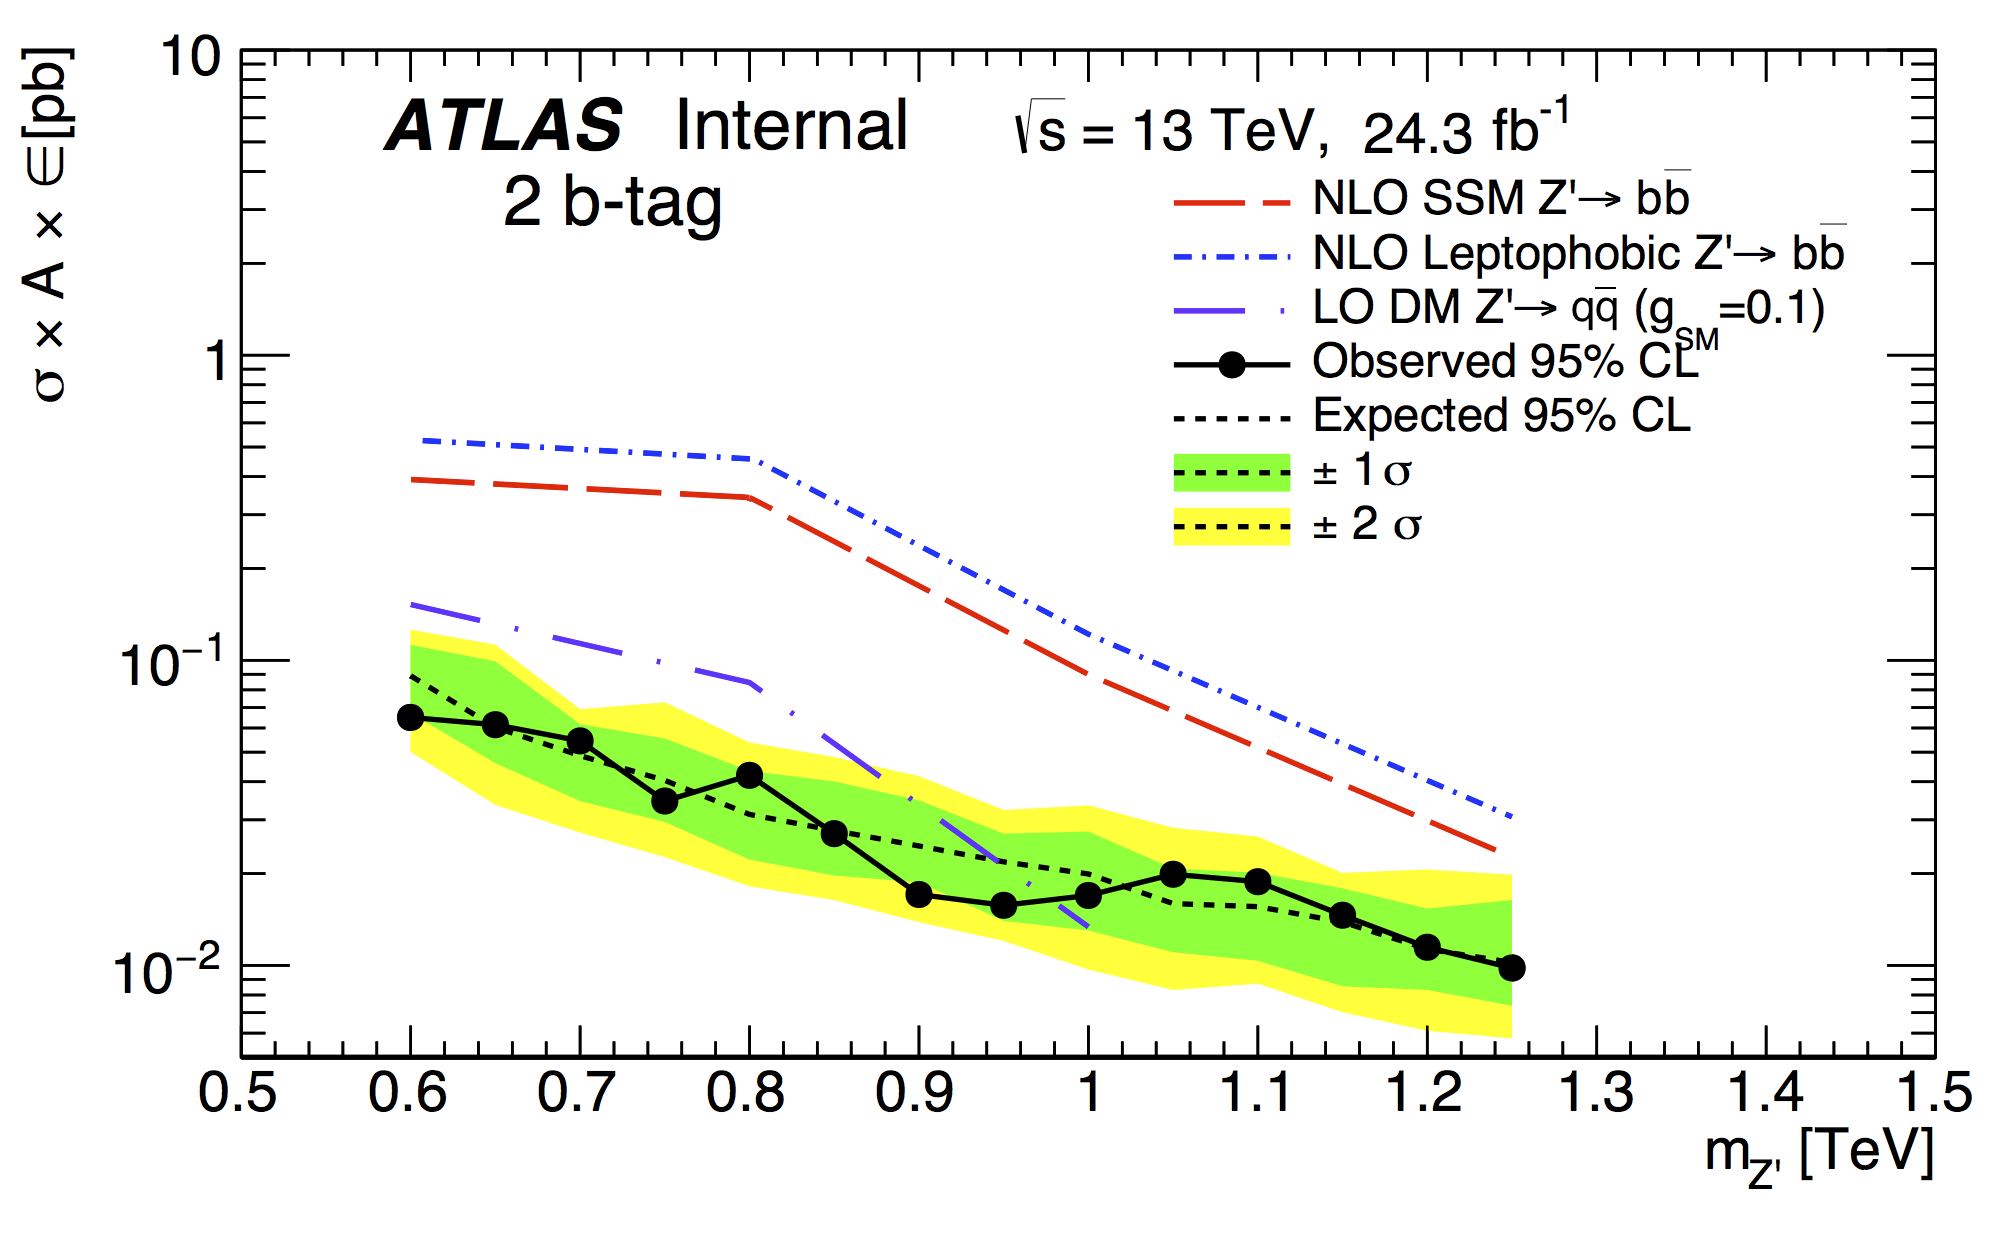
\includegraphics[width=0.8\linewidth, angle=0]{figs/Dibjet/LowMass/lim-lowmass_zprime_mjjcut.png}
%  \caption[95\% credibility level upper limits on
%           cross-section times acceptance times tagging efficiency
%           ($\sigma\,\text{x}\,\mathit{A}\,\text{x}\,\epsilon$)
%           for the $Z'$ boson and as a function of generated mass using the \lm{} data-set.]
%          {95\% credibility level upper limits on cross-section times acceptance times tagging efficiency
%            ($\sigma\,\text{x}\,\mathit{A}\,\text{x}\,\epsilon$)
%             for the $Z'$ boson and as a function of generated mass using the \lm{} data-set.
%             The observed limit is shown by the solid black line, the expected limit is shown by the dotted black line
%             and the 1 and 2 $\sigma$ uncertainty bands on the expected limit are shown by the green and yellow bands.
%             The theoretical prediction of $\sigma\,\text{x}\,\mathit{A}\,\text{x}\,\epsilon$
%             for the Sequential Standard Model (SSM) and leptophobic Z' models decaying to a pair $b$-quarks
%             and the DM $Z'$ boson decaying to $u$, $d$, $s$, $c$ and $b$ quarks are overlaid~\cite{dibjet-full_int}.
%          }
%  \label{fig:lim-lowmass_benchmark}
%\end{figure}

\begin{figure}[!ht]
  \centering
  \captionsetup[subfigure]{aboveskip=0pt,justification=centering}
  \subcaptionbox{SSM and Leptophobic $Z'$ Boson\vspace{12pt}} {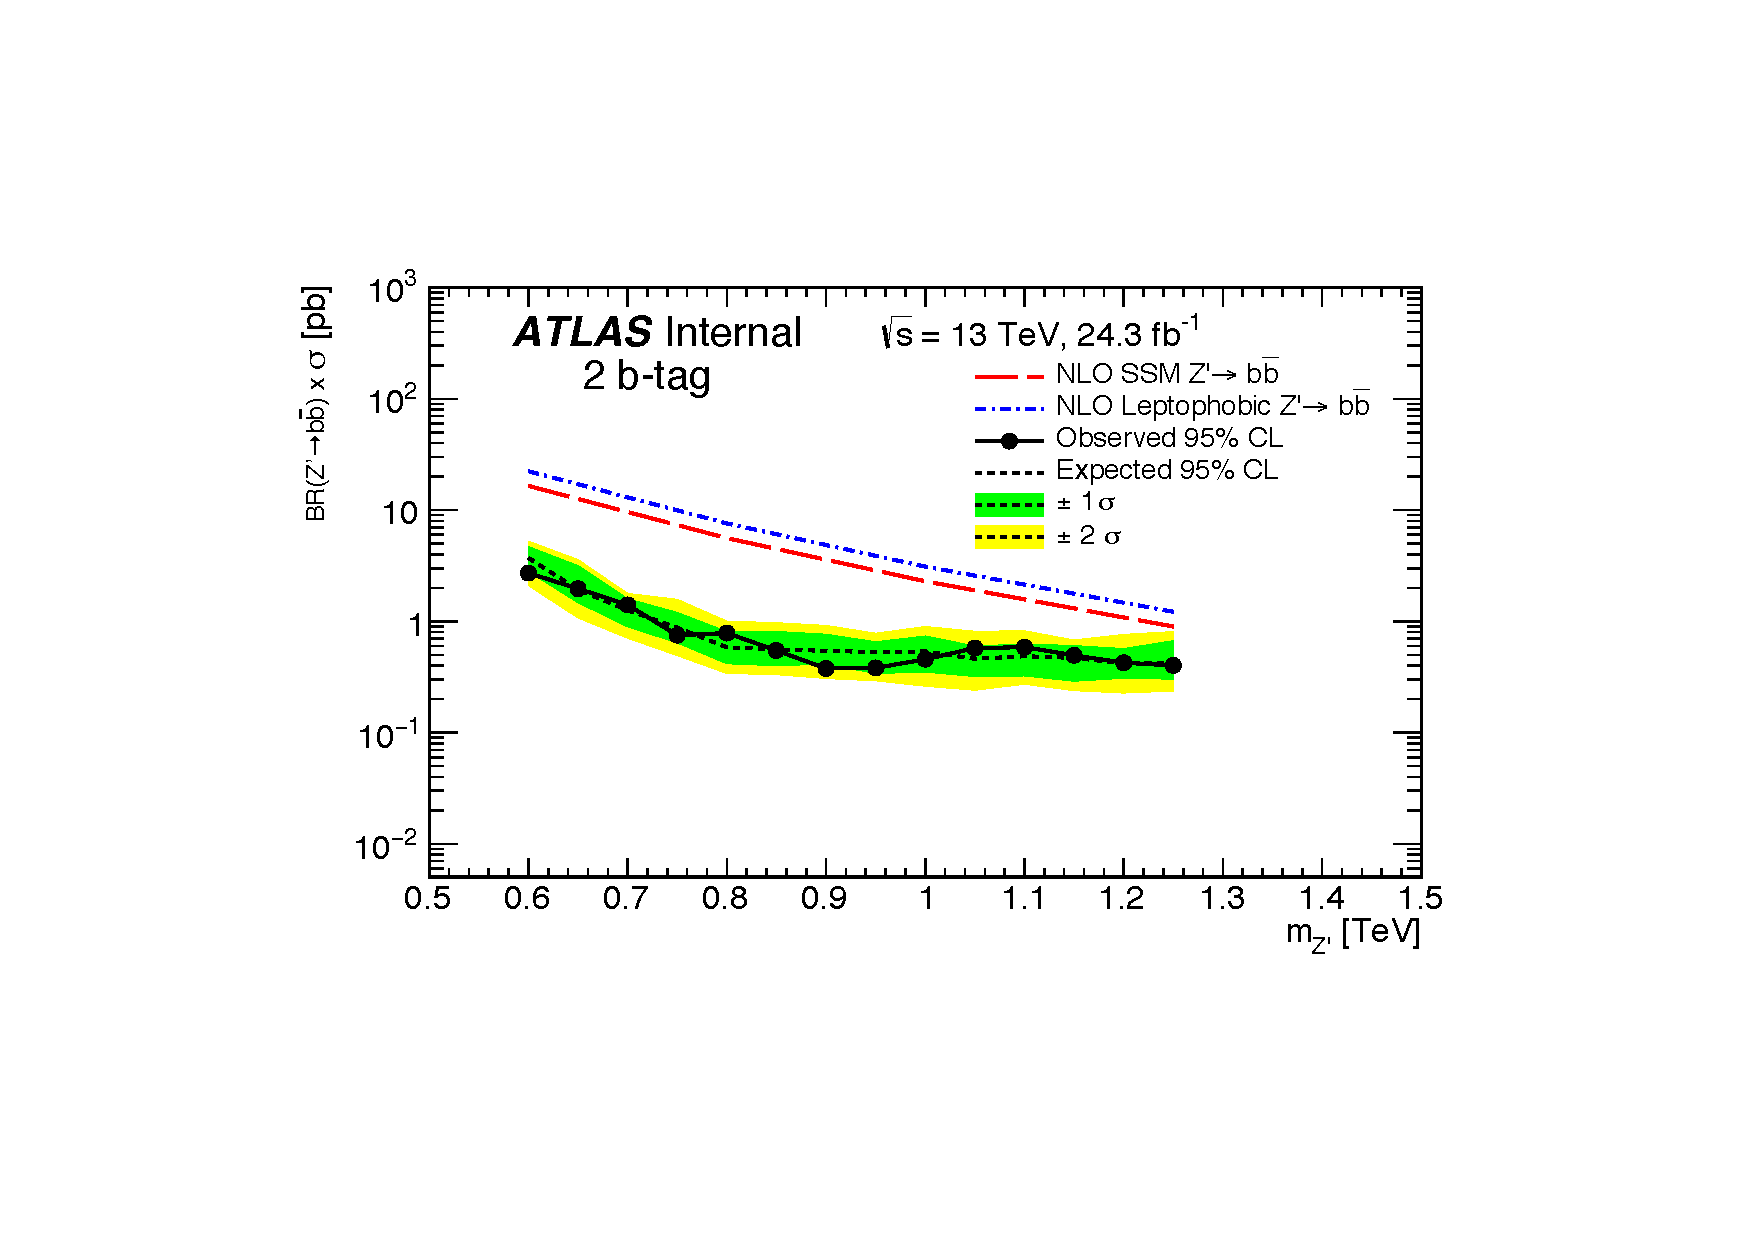
\includegraphics[width=0.9\linewidth, angle=0]{figs/Dibjet/LowMass/lim-zprime_SSM_BR.pdf}\vspace{-4pt}}
  
  \subcaptionbox{DM $Z'$ Boson}                  {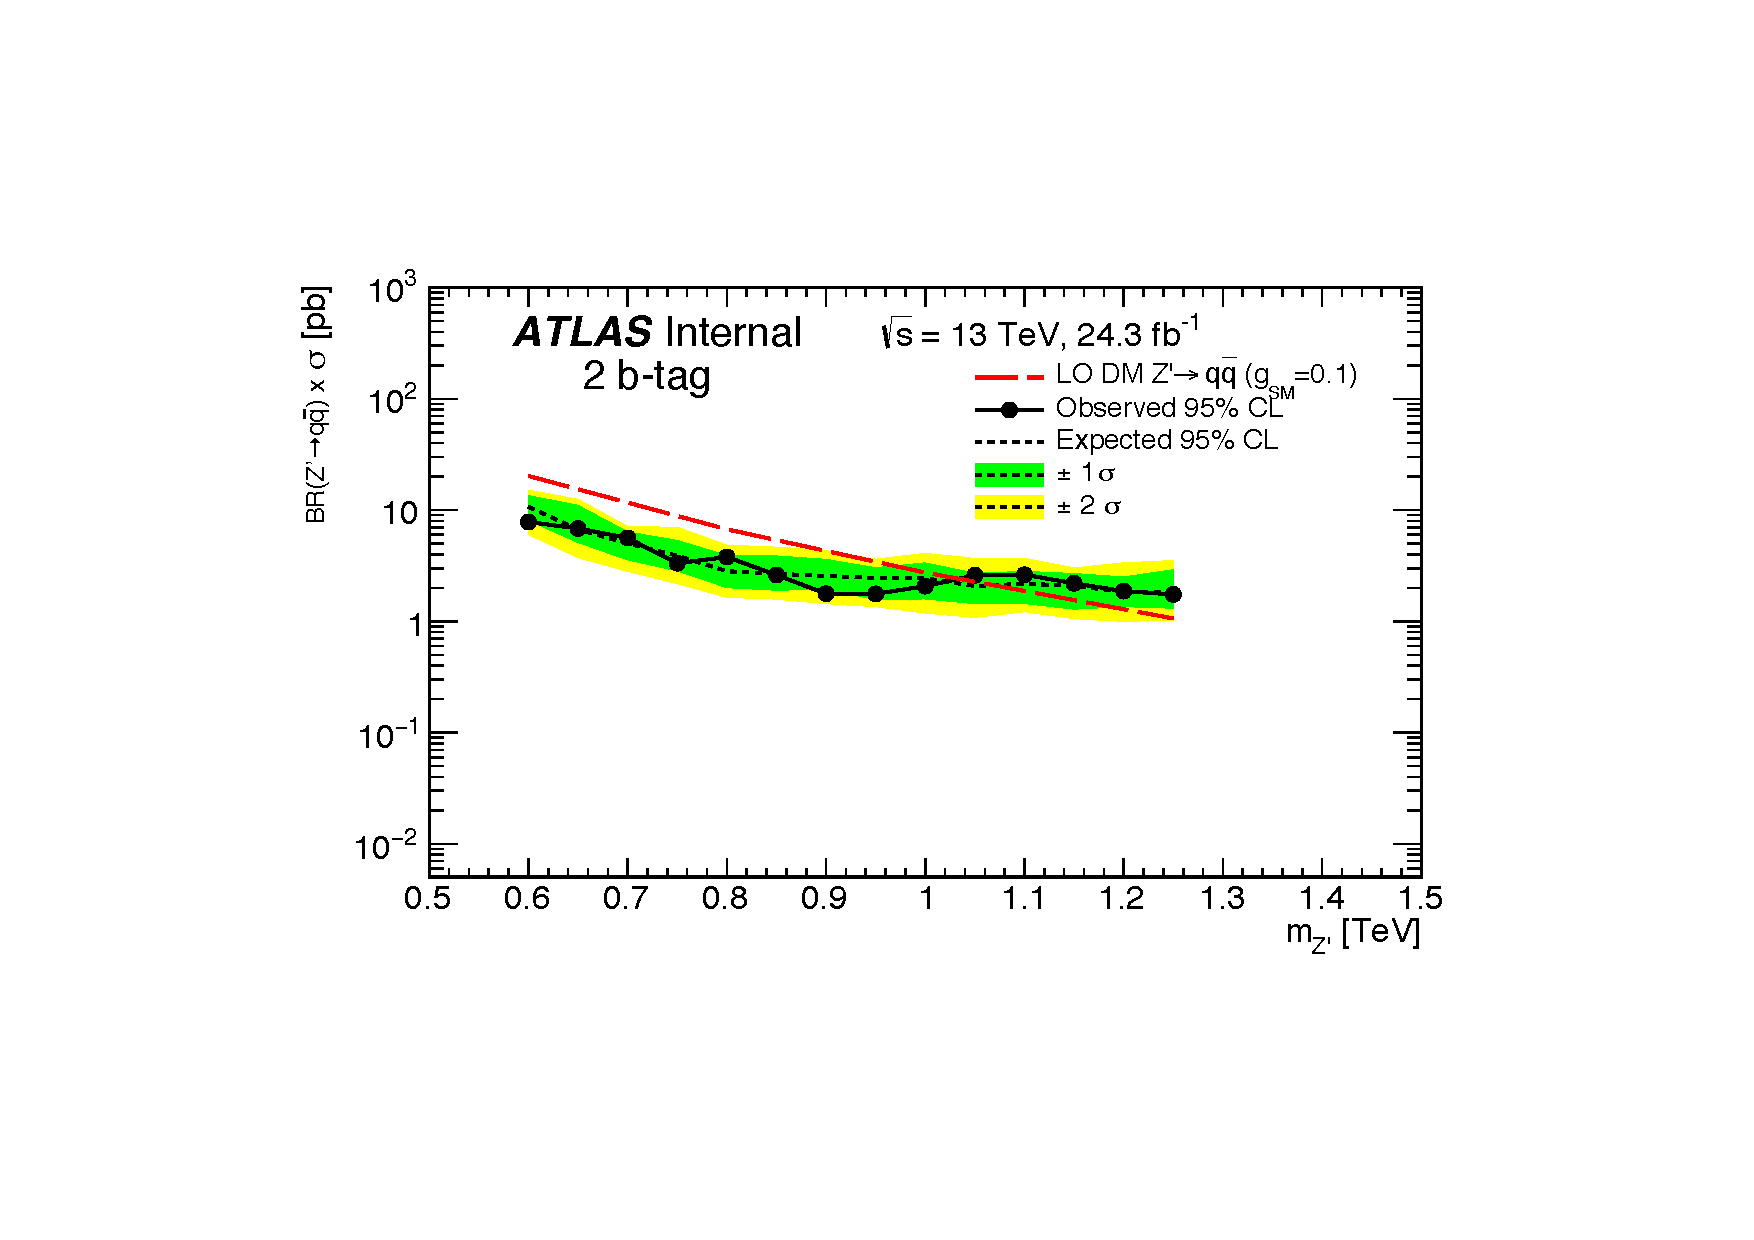
\includegraphics[width=0.9\linewidth, angle=0]{figs/Dibjet/LowMass/lim-zprime_DM_BR.pdf}}
  \caption
      [95\% credibility level upper limits on the product of cross-section and branching ratio 
        for the SSM, leptophobic and DM $Z'$ boson and as a function of generated mass using the \lm{} data-set.]
      {95\% credibility level upper limits on the product of
        cross-section and branching ratio ($\sigma\,\text{x}\,\mathit{BR}$)
        for (a) the Sequential Standard Model (SSM) and leptophobic $Z'$ boson decaying to a pair of $b$-quarks
        and (b) the DM $Z'$ boson decaying to a pair of $u$, $d$, $s$, $c$ or $b$ quarks
        as a function of generated mass using the \lm{} data-set.
        The observed limit is shown by the solid black line, the expected limit is shown by the dotted black line
        and the associated 1 and 2 $\sigma$ uncertainty bands on the expected limit are shown by the green and yellow bands.
        The theoretical predictions of $\sigma\,\text{x}\,\mathit{BR}$
        for the  SSM, leptophobic and DM $Z'$ models are overlaid~\cite{dibjet-full_int}.
      }
  \label{fig:lim-lowmass_benchmark}
\end{figure}

\clearpage

For the generic Gaussian limit setting phase there is a significant difference
with respect to the \summer{} data-set analysis.
In the \summer{} data-set analysis a signal template with a Gaussian distribution in dijet mass is used,
whilst for the \lm{} data-set analysis a signal template with a Gaussian distribution in the truth mass distribution is used.
The truth mass is defined as the invariant mass of the leading and subleading truth jets,
using the definition of truth jet from Section~\ref{sec:obj-jets_calib}.
Limits placed on a Gaussian signal shape in truth mass can be interpreted for a range of signal models without
further information on the dijet mass resolution of the detector.

The centre of the truth mass Gaussian distribution is referred to as the generated mass,
the generated mass points used are in the range 0.65--1.45~TeV with a spacing of 0.05~TeV.
The lowest generated mass considered by the Gaussian limits is 0.65~TeV,
such that the majority of the signal events have a dijet mass above the 566~GeV requirement in the \lm{} data-set event selection.
The width of the Gaussian distributions are 15\%, 10\%, 7\%, 5\%, 3\% and 0\% of the generated mass;
a Gaussian distribution with a 0\% width is a Dirac delta peak.
The transformation of the signal templates from truth mass to dijet mass is performed using
transfer matrices calculated in a Monte-Carlo simulated QCD dijet sample,
following the procedure outlined in~\cite{dijet-mori17_paper}.
The Gaussian signal with a 0\% width in truth mass will have
a width of the mass resolution of the detector in dijet mass.

For the Gaussian limit setting phase, the sources of systematic uncertainties
are the luminosity uncertainty,
the background modelling uncertainties and a flat 5\% uncertainty to cover
the JES, JER and $b$JES systematic uncertainties.
Other systematic uncertainties are not included in the preliminary limits,
as these are found to have a small effect on the upper limit relative to the jet energy uncertainties.
This is because the jet energy uncertainties cause uncertainties on the dijet mass of a simulated event and
therefore can significantly affect the shape of the dijet mass signal template.

Figure~\ref{fig:lim-lowmass_gauss} shows the observed 95\% credibility upper limits set 
on the product of cross-section, detector acceptance, tagging efficiency and branching ratio,
$\sigma\,\text{x}\,\mathit{A}\,\text{x}\,\epsilon\,\text{x}\,\mathit{BR}$,
for the full range of Gaussian signals described above.
For the Gaussian signal with 0\% width in truth mass, which corresponds to the detector resolution in dijet mass,
the expected limits are shown by the dotted lines and the associated 1~and~2~$\sigma$ uncertainty bands are shown in green and yellow.
The results have not yet been published so should be considered as preliminary.

For the \lm{} data-set it is anticipated that an upper limit will be placed on the $\sigma\,\text{x}\,\mathit{A}\,\text{x}\,\epsilon\,\text{x}\,\mathit{BR}$
for a generic Gaussian signal ranging from 0.05 to 0.003 pb in the mass range 0.65~to~1.45~TeV.

\begin{figure}[!ht]
  \begin{center}
    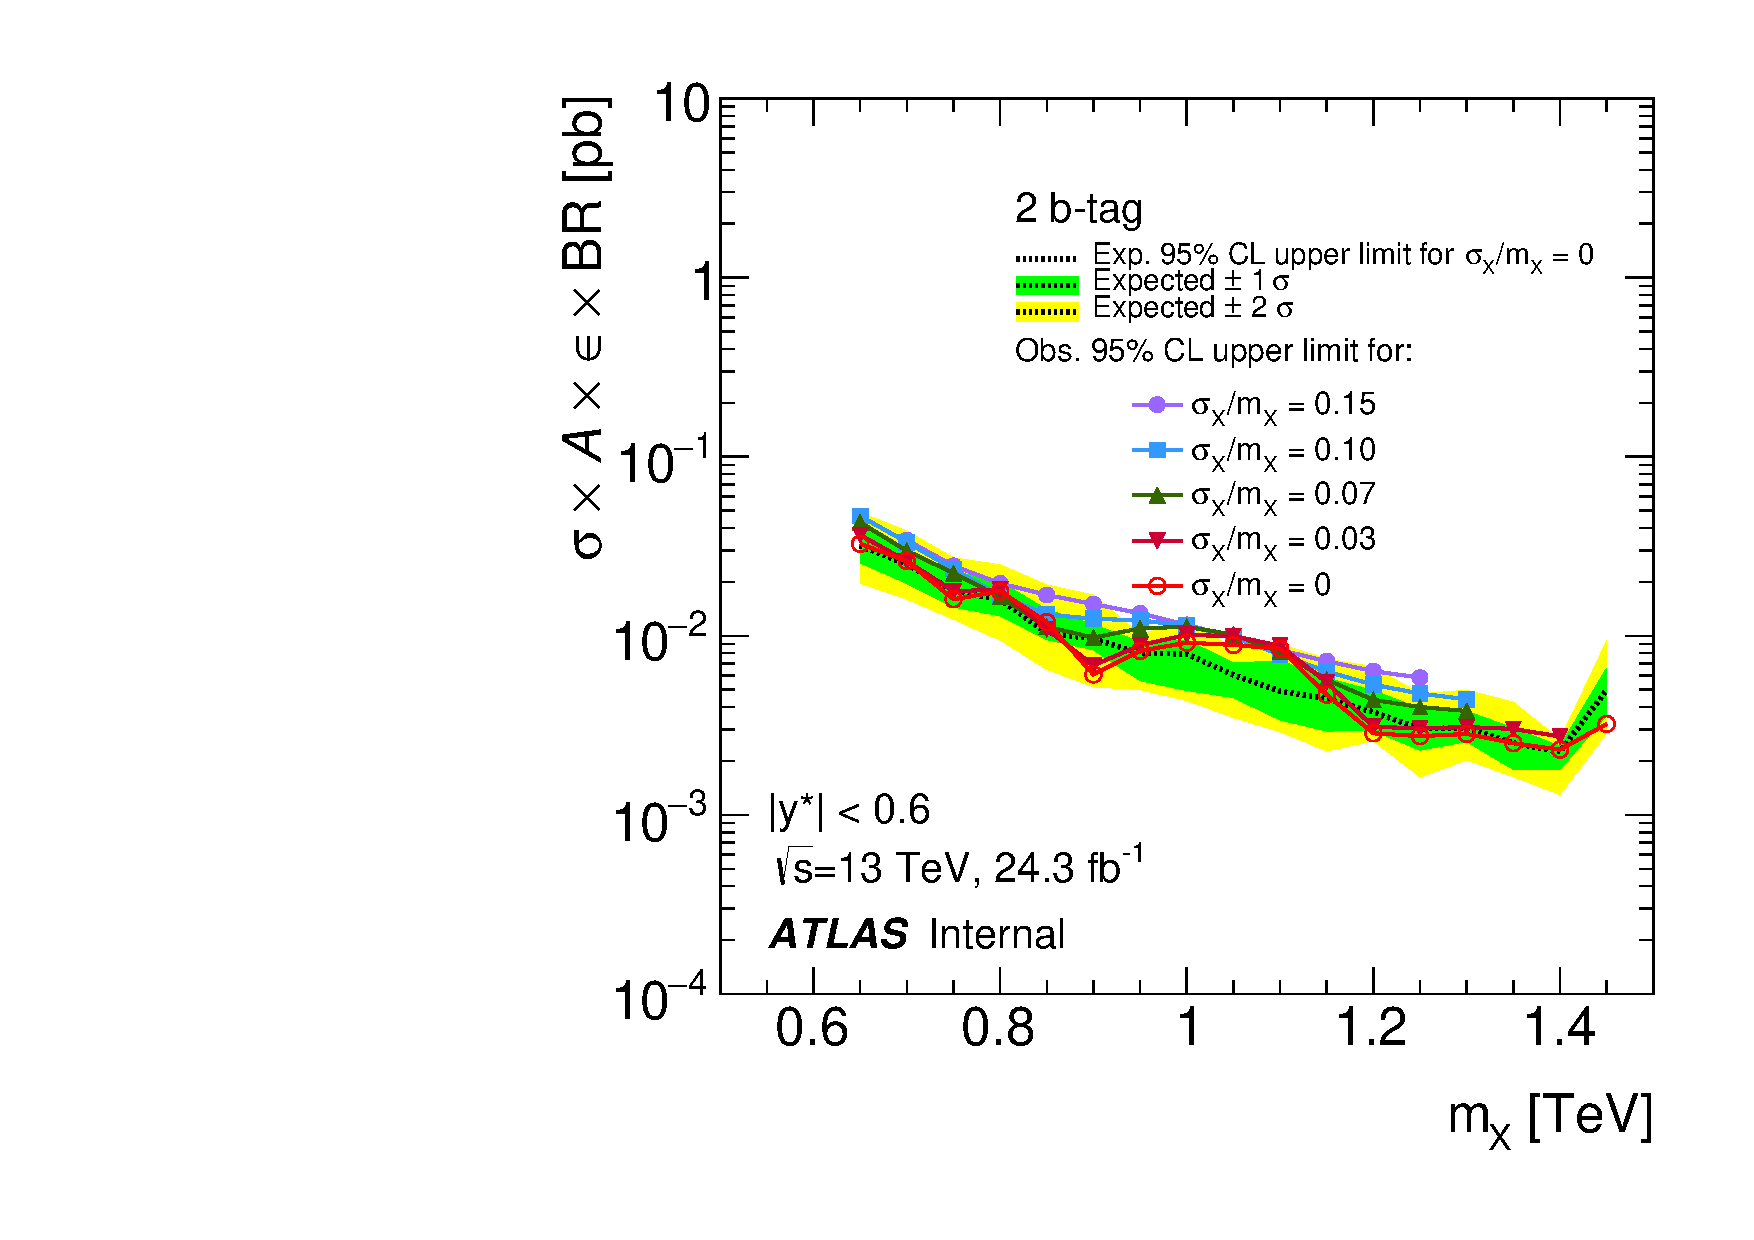
\includegraphics[width=0.9\linewidth, angle=0]{figs/Dibjet/lowmass/lim-gaussian.pdf}
  \vspace{-1.5em}
  \end{center}
  \caption[95\% credibility upper limits
    on the product of cross-section, detector acceptance, tagging efficiency and branching ratio
    for Gaussian signals using the \lm{} data-set.]
  {95\% credibility observed upper limits
    on the product of cross-section, detector acceptance, tagging efficiency and branching ratio,
    $\sigma\,\text{x}\,\mathit{A}\,\text{x}\,\epsilon\,\text{x}\,\mathit{BR}$,
    for Gaussian signals using the \lm{} data-set as a function of generated mass ($m_X$) are shown by the solid lines.
    The signal templates are a Gaussian distribution in truth mass with
    widths of 15\%, 10\%, 7\%, 5\%, 3\% and 0\% of the generated mass.
    The Gaussian distribution with 0\% width in truth mass represents the width of the detector resolution in dijet mass.
    Also shown are the expected 95\% credibility expected upper limit on the Gaussian signal shape with a 0\% width (dotted line)
    and the associated 1 and 2~\sigma{} uncertainty bands (green and yellow)~\cite{dibjet-full_int}.
  }
  \label{fig:lim-lowmass_gauss}
\end{figure}
